\documentclass[11pt]{article}
%% Packages:

\usepackage{amsmath}
\usepackage[document]{ragged2e}
\usepackage{titlesec}
\usepackage{float}
\usepackage{graphicx}
\usepackage{caption}
\usepackage{subcaption}
\usepackage[dvipsnames]{xcolor}
\usepackage[T1]{fontenc}
\usepackage{helvet}
\usepackage[hidelinks]{hyperref}
\usepackage[margin=2cm]{geometry}
\usepackage{amssymb}
\usepackage{enumitem}
\usepackage{comment}
\usepackage{soul}

%% Personalized adjustements: 

% Math operator:
\DeclareMathOperator{\sech}{sech}

% VUB colors: 
\definecolor{orange}{RGB}{234, 82, 0} 
\definecolor{blue}{RGB}{26, 55, 101}

% Margins:
\addtolength{\skip\footins}{0.3 cm}
\renewcommand*\footnoterule{}

% Adjustement of section, subsection & subsubsection: 

\titleformat{\section}[block]
{\normalfont\Large\bfseries \fontfamily{phv}\selectfont \color{orange}}
{\thesection}{0.5cm}{}

\titleformat{\subsection}[block]
{\normalfont\large\bfseries \fontfamily{phv}\selectfont \color{blue}}
{\thesubsection}{0.5cm}{}

\titleformat{\subsubsection}[block]
{\normalfont\small\bfseries \fontfamily{phv}\selectfont \color{blue}}
{\thesubsubsection}{0.5cm}{} 
\usepackage{setspace}
\usepackage{graphicx}
\usepackage{subcaption}
\usepackage{parskip} 
\usepackage{indentfirst} 
\graphicspath{{Images/}}
\usepackage{float} 
\usepackage{amsmath}
\onehalfspacing

\begin{document}
	\justifying 
	\pagenumbering{roman}
	\begin{titlepage}
	\begin{center}
            \begin{figure}
                \centering
                
\includegraphics[scale=0.3]{Images/logo.png}
            \end{figure}
		\vspace*{\fill}
            \normalsize
            {\fontfamily{phv}\selectfont
            \textcolor{blue}{\textbf{ELEC-H401}}}\\
            \vspace{0.2cm}
		\Huge
            {\fontfamily{phv}\selectfont
            \textcolor{orange}{Design and Simulation of a DVB-C Transmission Chain}}\\
        \end{center}
	\begin{center}	
		\vspace{0.5cm}
            \Large
            {\fontfamily{phv}\selectfont
			\textcolor{blue}{\textbf{Hadislam Satouev\\
                                 	 Cédric Sipakam
             }}}\\
	\end{center}
        \vspace*{\fill}
        \begin{FlushRight}
            {\fontfamily{phv}\selectfont
            \textcolor{orange}{Professor}}\\
            {\fontfamily{phv}\selectfont
            \textcolor{blue}{François Horlin}}\\
            \vspace{0.6cm}
            {\fontfamily{phv}\selectfont
            \textcolor{orange}{Teaching Assistants}}\\
            {\fontfamily{phv}\selectfont
            \textcolor{blue}{
                ....\\
                 ....
            }}\\
            \vspace{0.6cm}
            {\fontfamily{phv}\selectfont
            \textcolor{orange}{Academic Year}}\\
            {\fontfamily{phv}\selectfont
            \textcolor{blue}{2024 - 2025}}\\
            \vspace{0.6cm}
            {\fontfamily{phv}\selectfont
            \textcolor{orange}{Faculty}}\\
            {\fontfamily{phv}\selectfont
            \textcolor{blue}{Electrical Engineering}}
        \end{FlushRight}



\end{titlepage} 
	\tableofcontents
	\newpage
	\listoffigures
	\newpage
        \pagenumbering{arabic}
	\section*{Introduction}{\addcontentsline{toc}{section}{Introduction}}
	This project focuses on designing and simulating a Digital Video Broadcasting Cable transmission chain using Matlab.
	The main goal is to model and analyze the components of a typical modem. The first part of this project includes establishing an optimal communication chain over an ideal Additive White Gaussian Noise channel, mapping the signal into symbols, Nyquist filtering, and evaluating the performance of the system through Bit Error Rate simulations. The second part revolves around the design and assessment of time and frequency synchronization algorithms. This encompasses evaluating the impact of synchronization errors such as carrier phase offset, frequency offset, and sample time shift. The algorithms used for this purpose are the Gardner Algorithm for timing recovery, and a differential cross-correlator for joint frame and frequency acquisition. Afterwards, their effectiveness is demonstrated through convergence analysis and residual error evaluation. Finally, the project aims to validate the simulated chain through real-life experimentation on a Hybrid Fiber-Coax setup using Adalm-Pluto hardware, and to compare the simulated performance with experimental observations.
	
	
	\section{Optimal Communication Chain over the Ideal Channel}
	Figure \ref{fig:com-chain} shows the simulated DVB-C baseband communication chain. The transmitter generates bits, maps them to QAM symbols, upsamples, and pulse-shapes them with a half-root Nyquist filter. The receiver uses a matched filter, then downsamples and demapps the symbols. In this project, Low-density parity-check (LDPC) coding is not implemented.
	
	\begin{figure}[H]
		\centering
		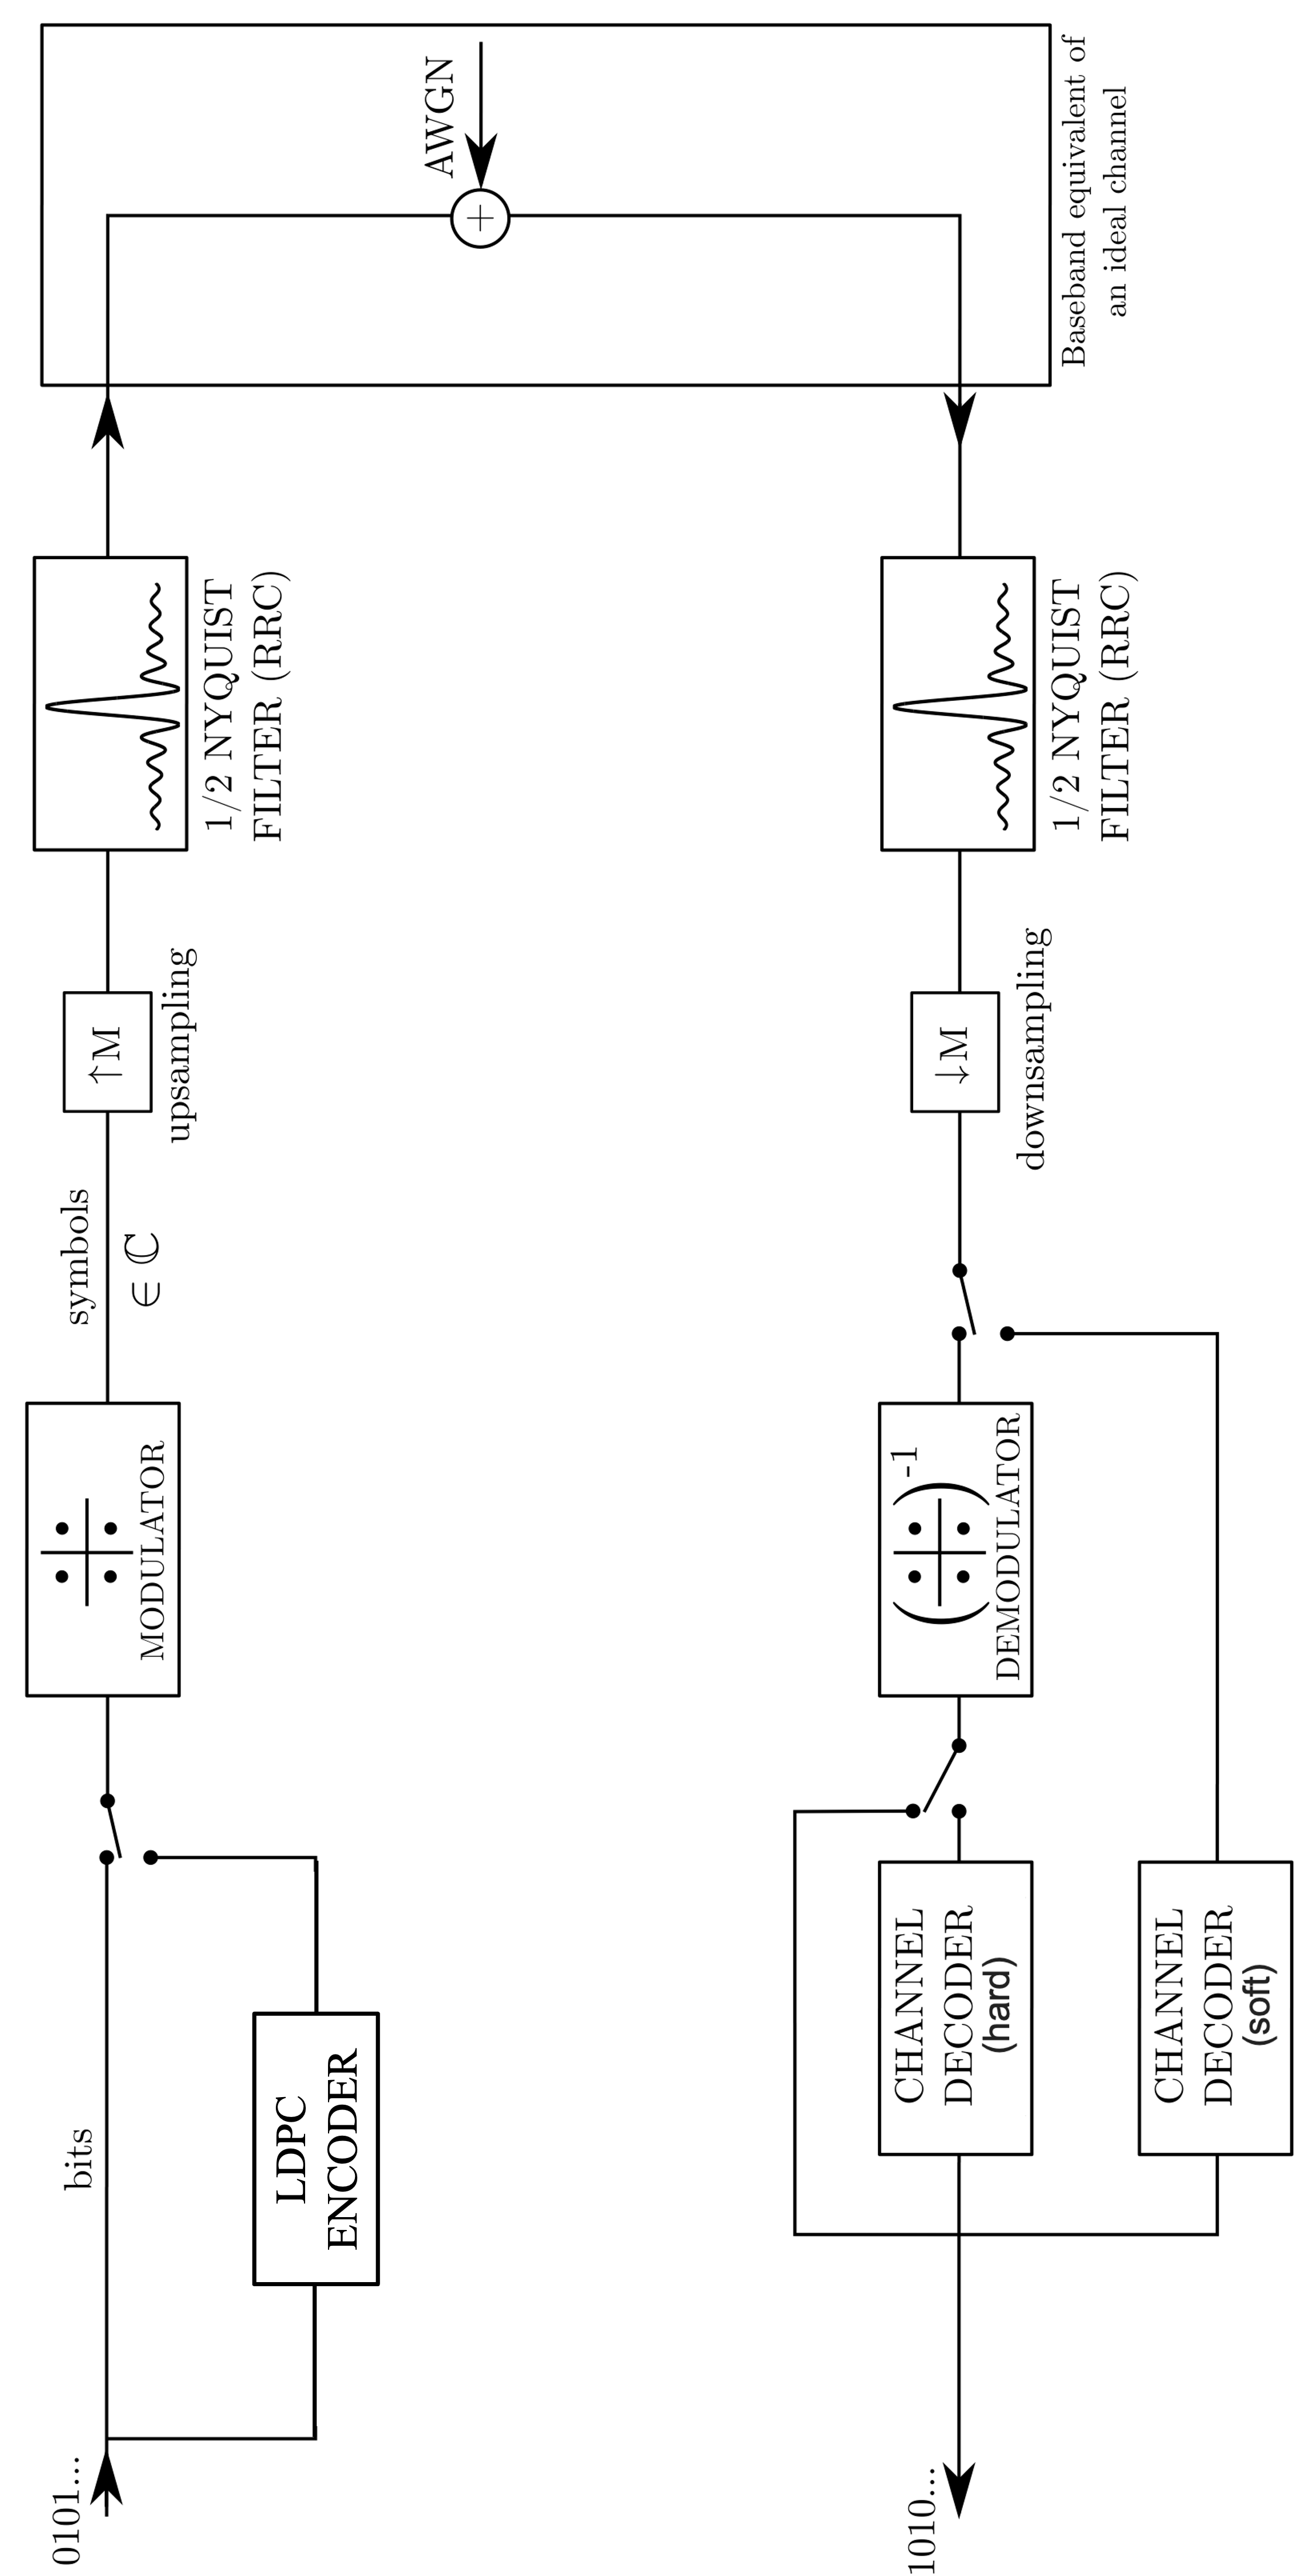
\includegraphics[angle=-90, width=0.6\linewidth]{Images/com-chain}
		\caption{Block diagram of the communication system.}
		\label{fig:com-chain}
	\end{figure}
	
	\subsection{Symbol Mapping and Demapping}
	Symbol mapping transforms random bits into complex symbols. The demapping process uses the Maximum Likelihood (ML) criterion to select the constellation symbol $\underline{s}_{m}$ that minimizes the Euclidean distance to the received sample $\underline{r}$:
	\begin{equation}
		\tilde{\underline{s}}_{m}^{\text{ML}} = \operatorname*{arg\,min}_{\underline{s}_{m}} \left(\sum_{k=1}^{K}(r_{k}-s_{mk})^{2}\right)
	\end{equation}
	This is equivalent to maximizing $\ln p(\underline{r}|\underline{s}_{m})$ for an AWGN channel.
	
	\subsection{Half-Root Nyquist Filter Design}
	Nyquist filtering employs a root-raised cosine (RRC) filter $g(t)$ at the transmitter for pulse shaping, and its matched version $g^*(-t)$ at the receiver. Their convolution, $h(t) = g(t) \otimes g^*(-t)$, satisfies the Nyquist criterion for zero Inter-Symbol Interference (ISI) at sampling intervals $T_{\text{symb}}$, meaning $h(kT_{\text{symb}}) \approx \delta[k]$. The RRC frequency response is $G(f) = \sqrt{H(f)}$, where $H(f)$ is the raised cosine (RC) filter response, given by:
	\begin{equation}
		H(f) = \begin{cases}
			T_{\text{symb}} & 0 \le |f| < \frac{1-\beta}{2T_{\text{symb}}} \\ 
			\frac{T_{\text{symb}}}{2} \left(1 + \cos\left[\frac{\pi T_{\text{symb}}}{\beta}\left(|f| - \frac{1-\beta}{2T_{\text{symb}}}\right)\right]\right) & \frac{1-\beta}{2T_{\text{symb}}} \le |f| \le \frac{1+\beta}{2T_{\text{symb}}} \\ 
			0 & |f| > \frac{1+\beta}{2T_{\text{symb}}}
		\end{cases}
	\end{equation}
	Figure \ref{fig:nyquist-filter-combined} shows the simulated $H(f)$ for $R_{\text{symb}} = 5 \text{ Msymb/s}$ and $\beta = 0.2$, confining the signal to a 6 MHz bandwidth, and $h(t)$ illustrating ISI cancellation at $kT_{\text{symb}}$.
	
	\begin{figure}[H]
		\centering
		\begin{subfigure}[t]{0.53\textwidth}
			\centering
			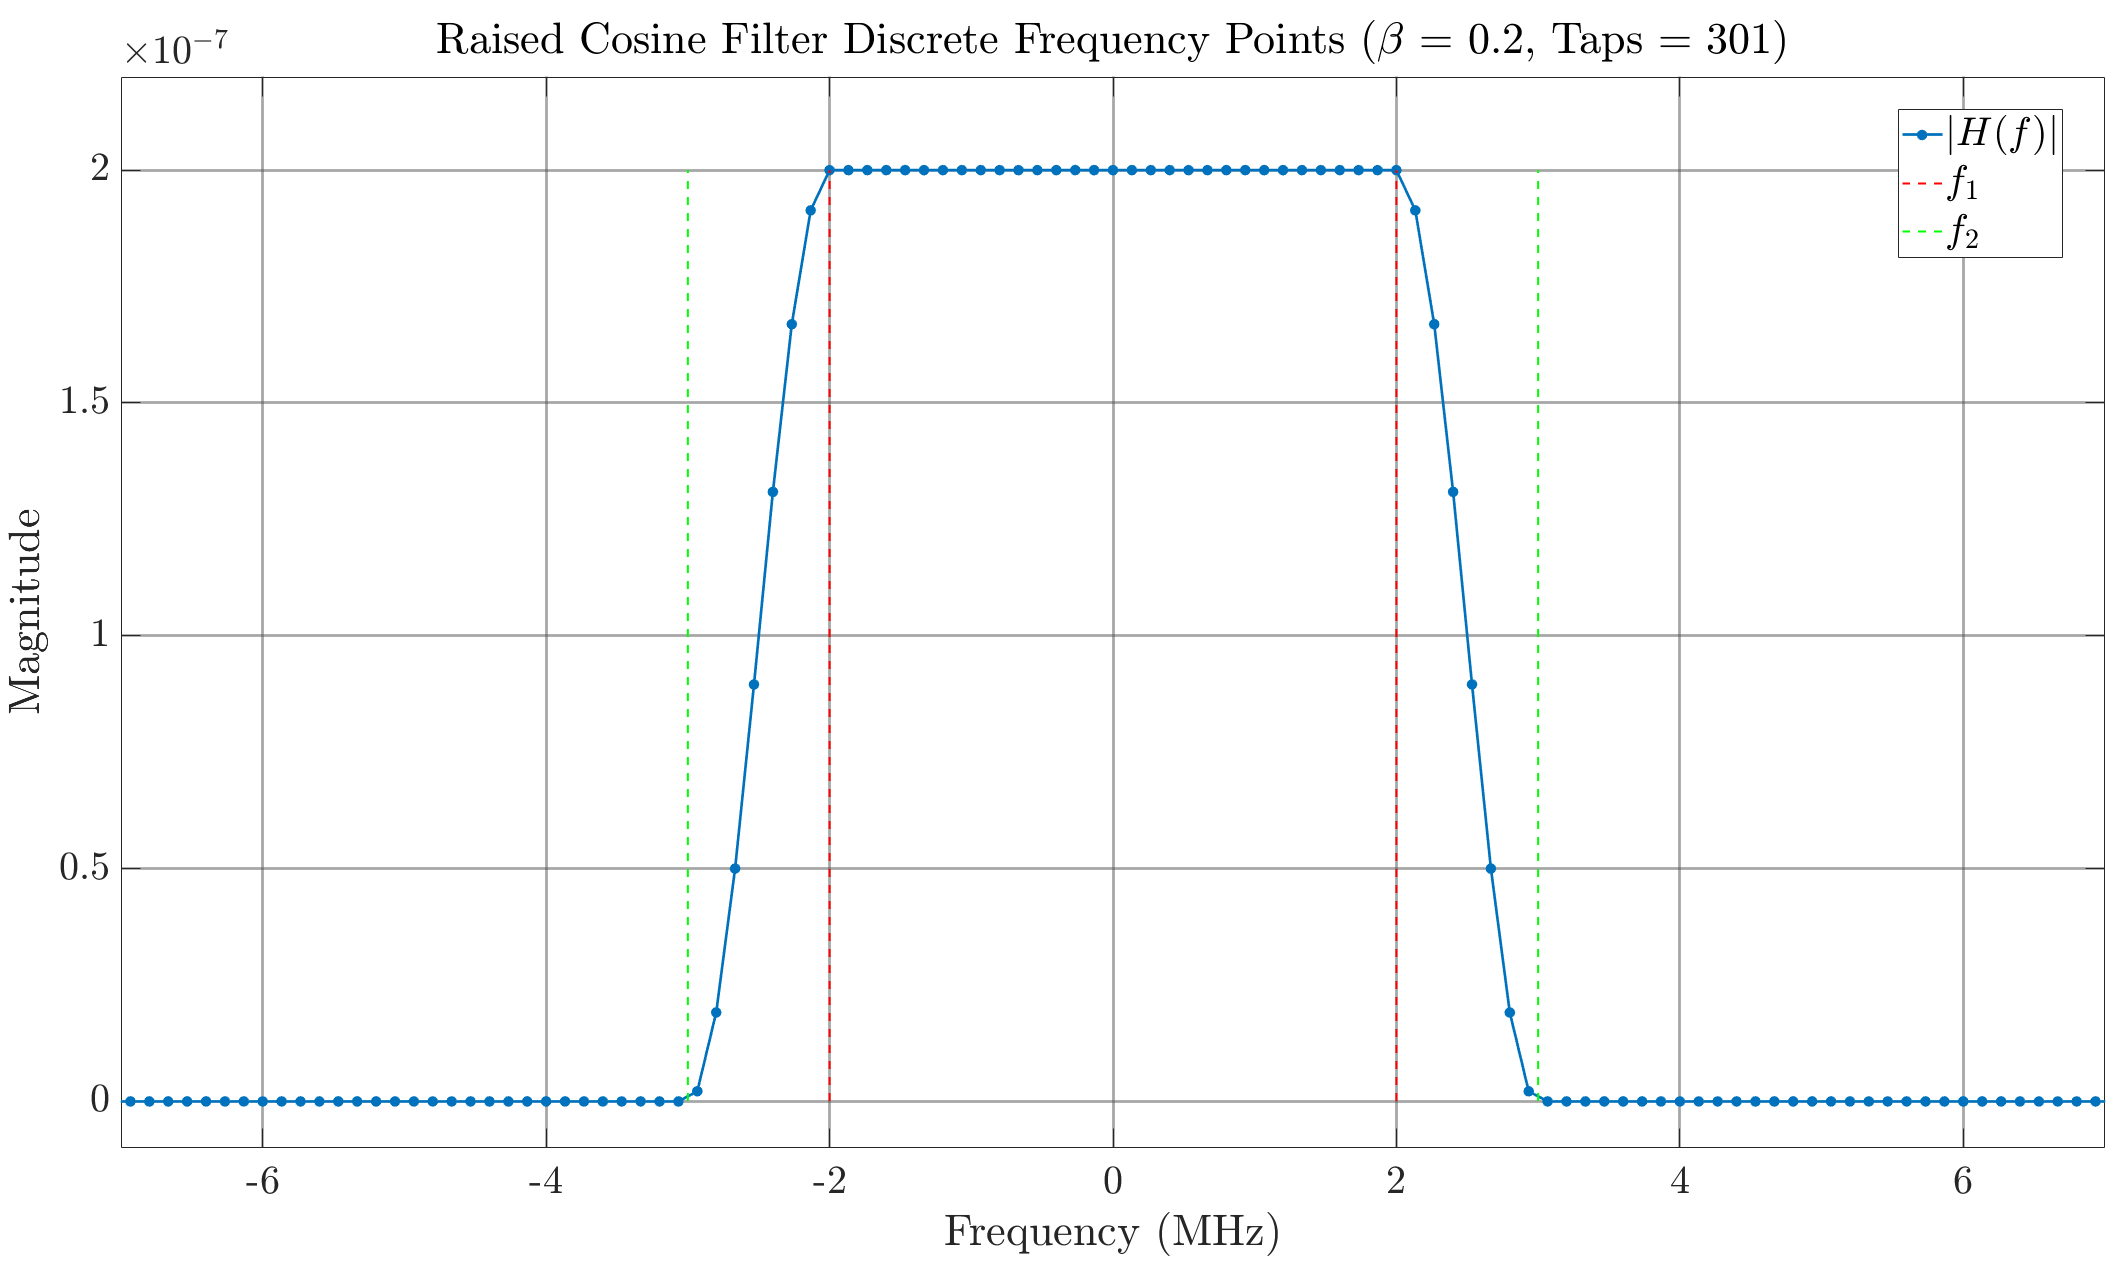
\includegraphics[width=\linewidth]{Images/h-rc-freq}
			\caption{RC Filter Frequency Response ($\beta = 0.2$).}
			\label{fig:h-rc-freq_compact}
		\end{subfigure}
		\hfill
		\begin{subfigure}[t]{0.46\textwidth}
			\centering
			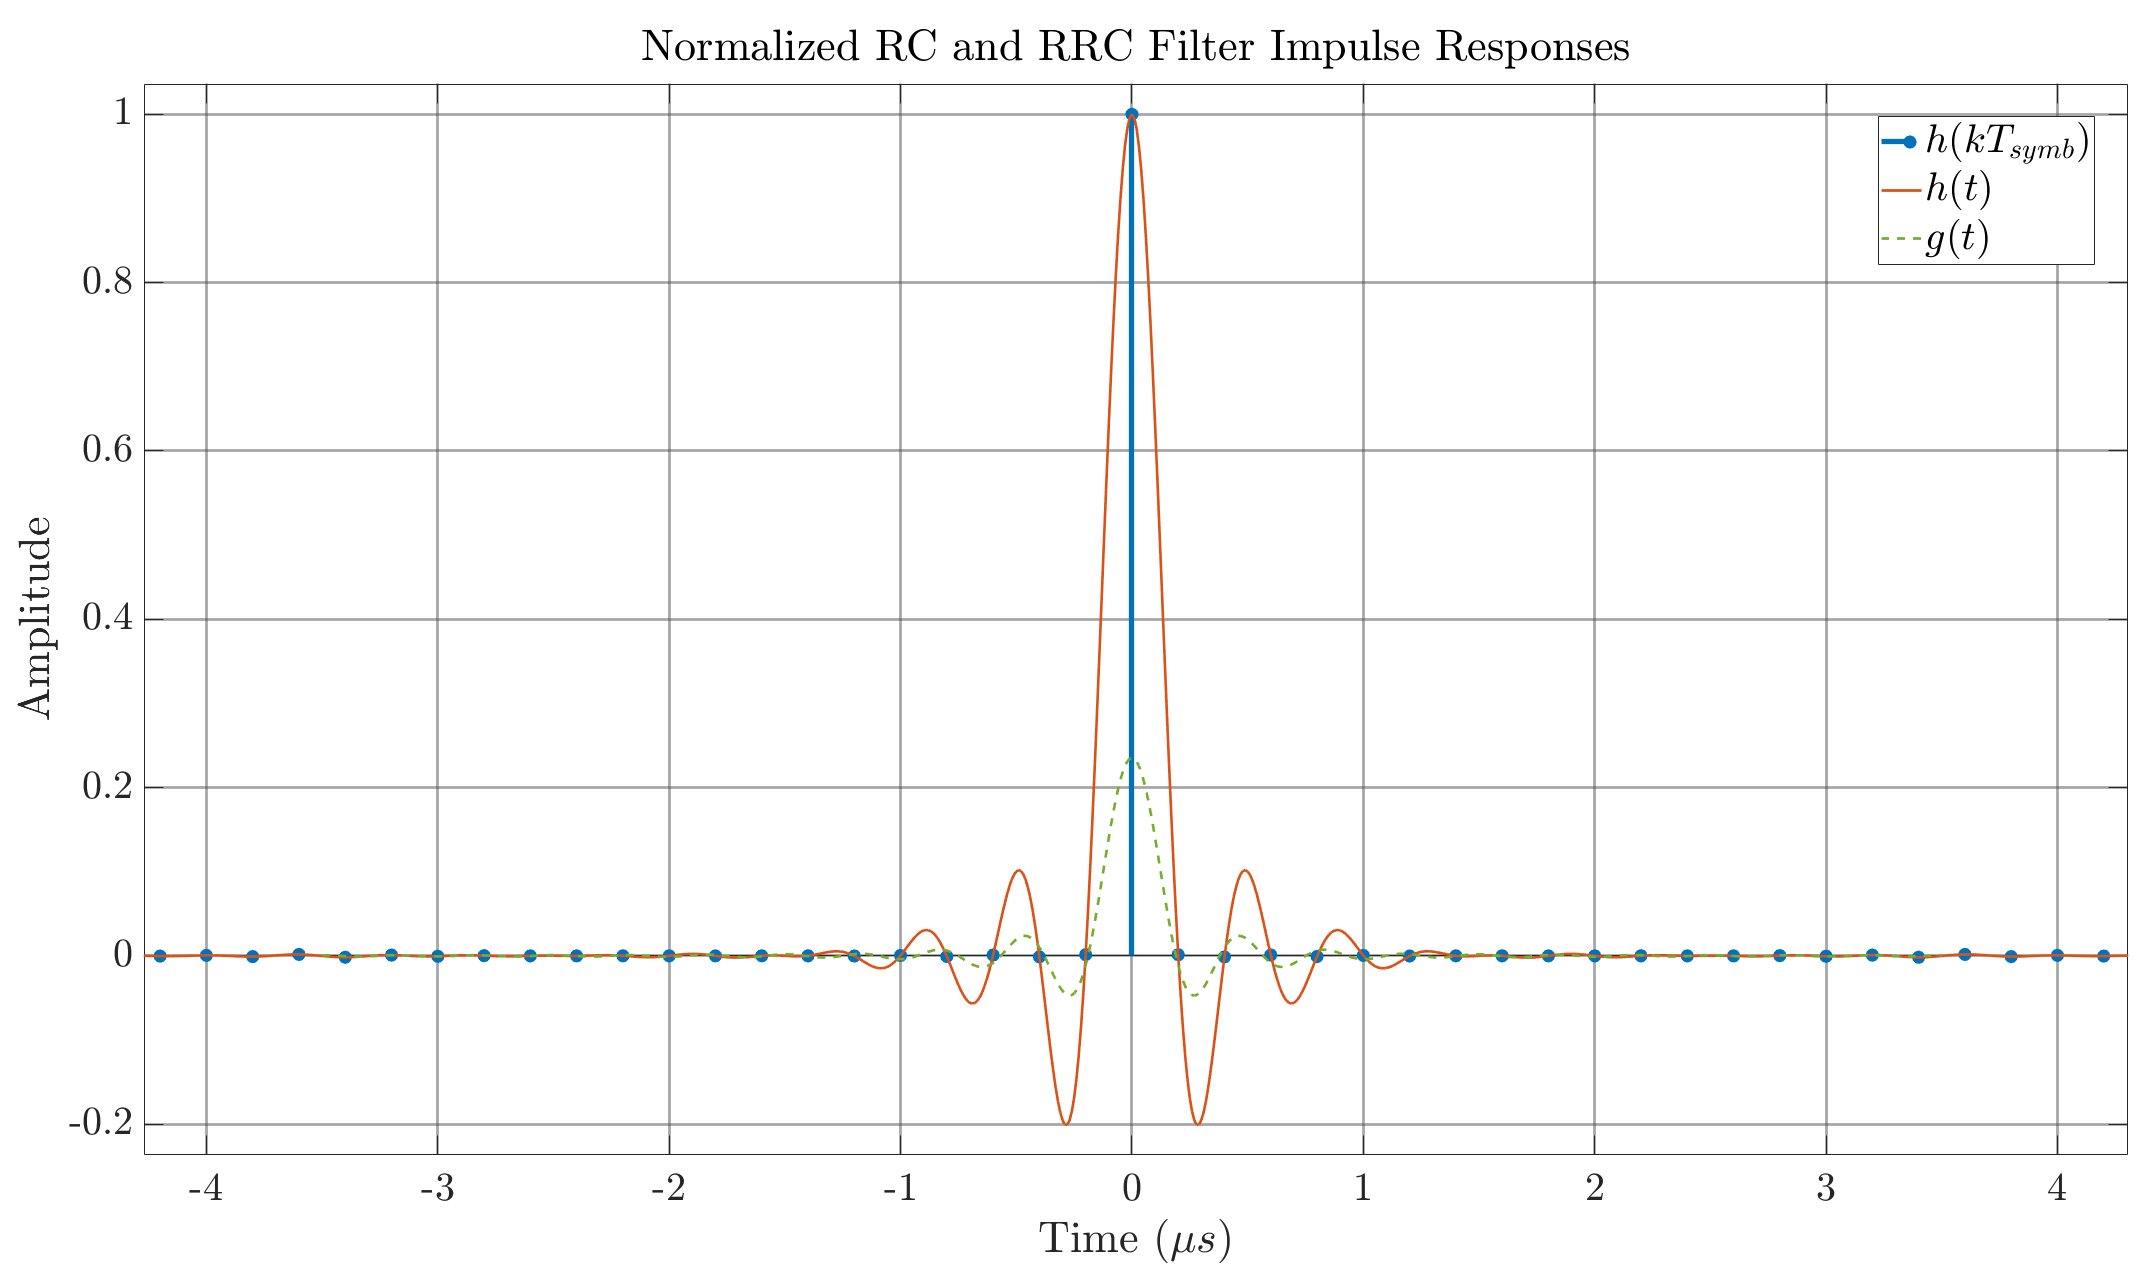
\includegraphics[width=\linewidth]{Images/h-rc}
			\caption{Normalized RC and RRC Impulse Responses.}
			\label{fig:h-rc_compact}
		\end{subfigure}
		\caption{Simulated Nyquist filter characteristics.}
		\label{fig:nyquist-filter-combined}
	\end{figure}
	
	\subsection{Noise Modeling and Performance Evaluation}
	AWGN $n(t)$ is added to the signal $s(t)$, so $r(t) = s(t) + n(t)$. After matched filtering and sampling, $y[k] = I[k] + n_o[k]$, where $n_o[k]$ is complex Gaussian noise with variance $N_0/2$ per component. System performance is measured by the Bit Error Rate (BER) as a function of $E_b/N_0$. The theoretical BER, denoted as $P_b$, for M-QAM is approximately:
	\begin{equation}
		P_b \approx \frac{4}{\log_2 M} \left(1 - \frac{1}{\sqrt{M}}\right) Q\left(\sqrt{\frac{3 (\log_2 M)^2}{M-1} \frac{E_b}{N_0}}\right)
	\end{equation}
	Figure \ref{fig:ber-mod_cont} validates theoretical BER curves. Higher-order QAMs achieve higher data rates but require more power. Figure \ref{fig:constellations-noise_cont} shows the effect of AWGN on 16-QAM symbols before and after matched filtering, the latter showing tighter clusters due to the Signal-to-Noise Ratio (SNR) maximization property of matched filtering.
	
	\begin{figure}[H]
		\centering
		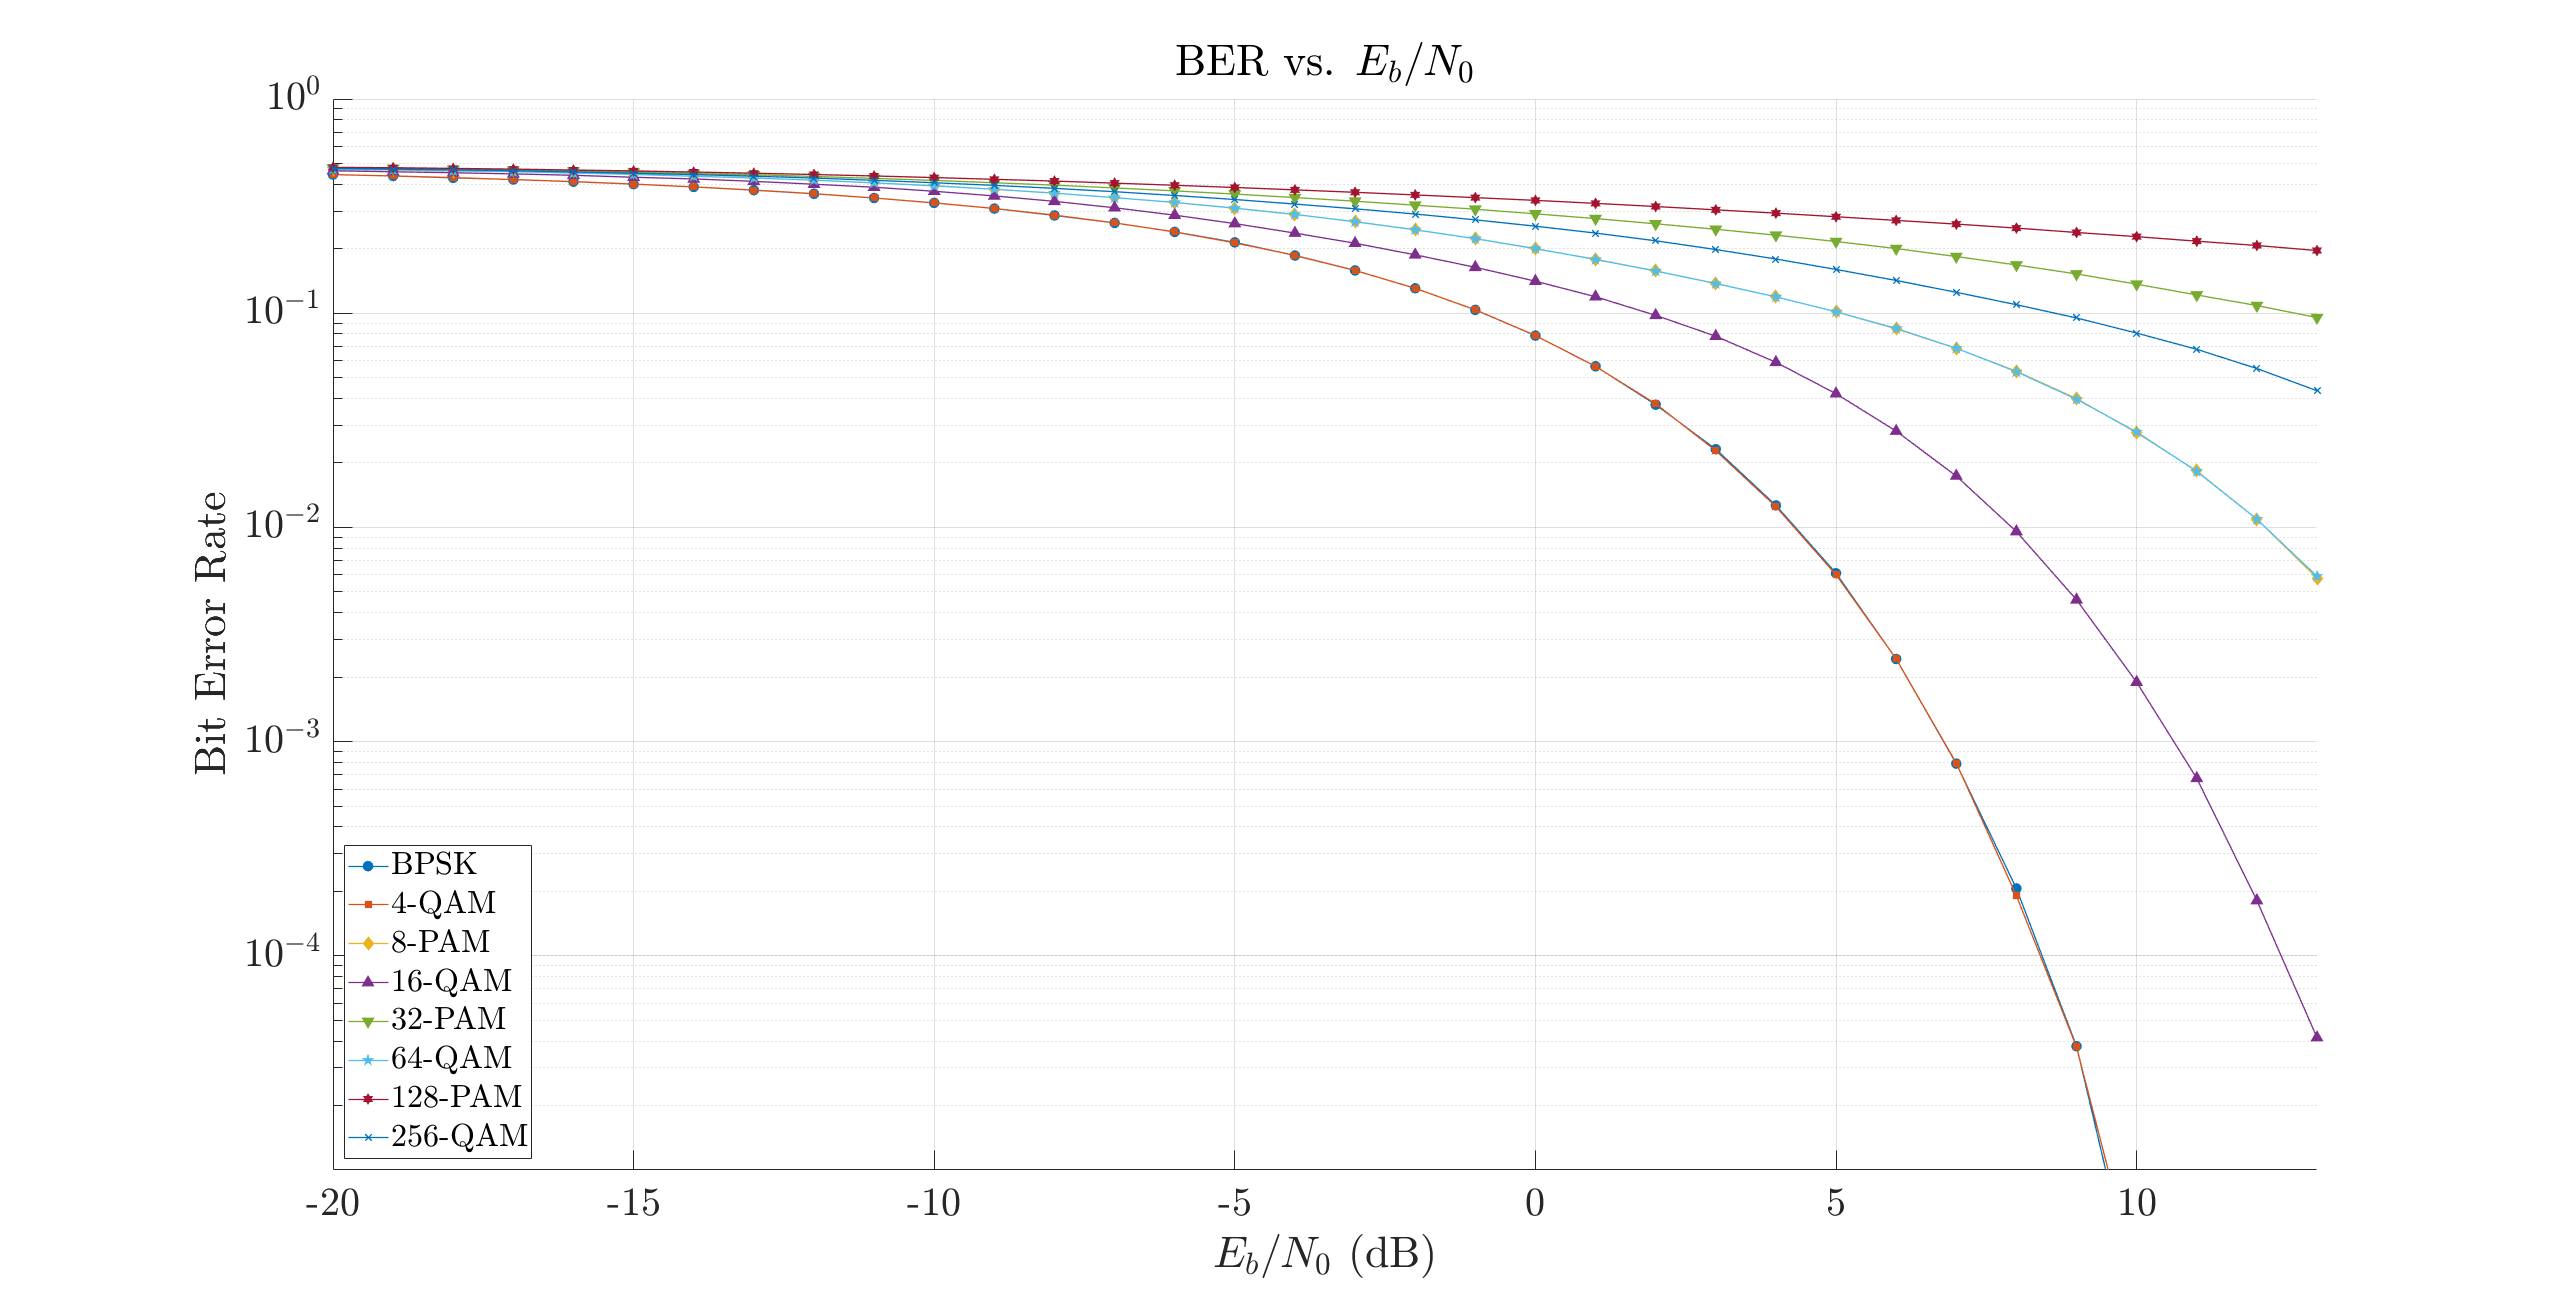
\includegraphics[width=0.7\linewidth]{Images/ber-mod.png}
		\caption{Simulated BER vs. $E_b/N_0$ for various modulation types.}
		\label{fig:ber-mod_cont}
	\end{figure}
	
	\begin{figure}[H]
		\centering
		\begin{subfigure}{0.4\textwidth}
			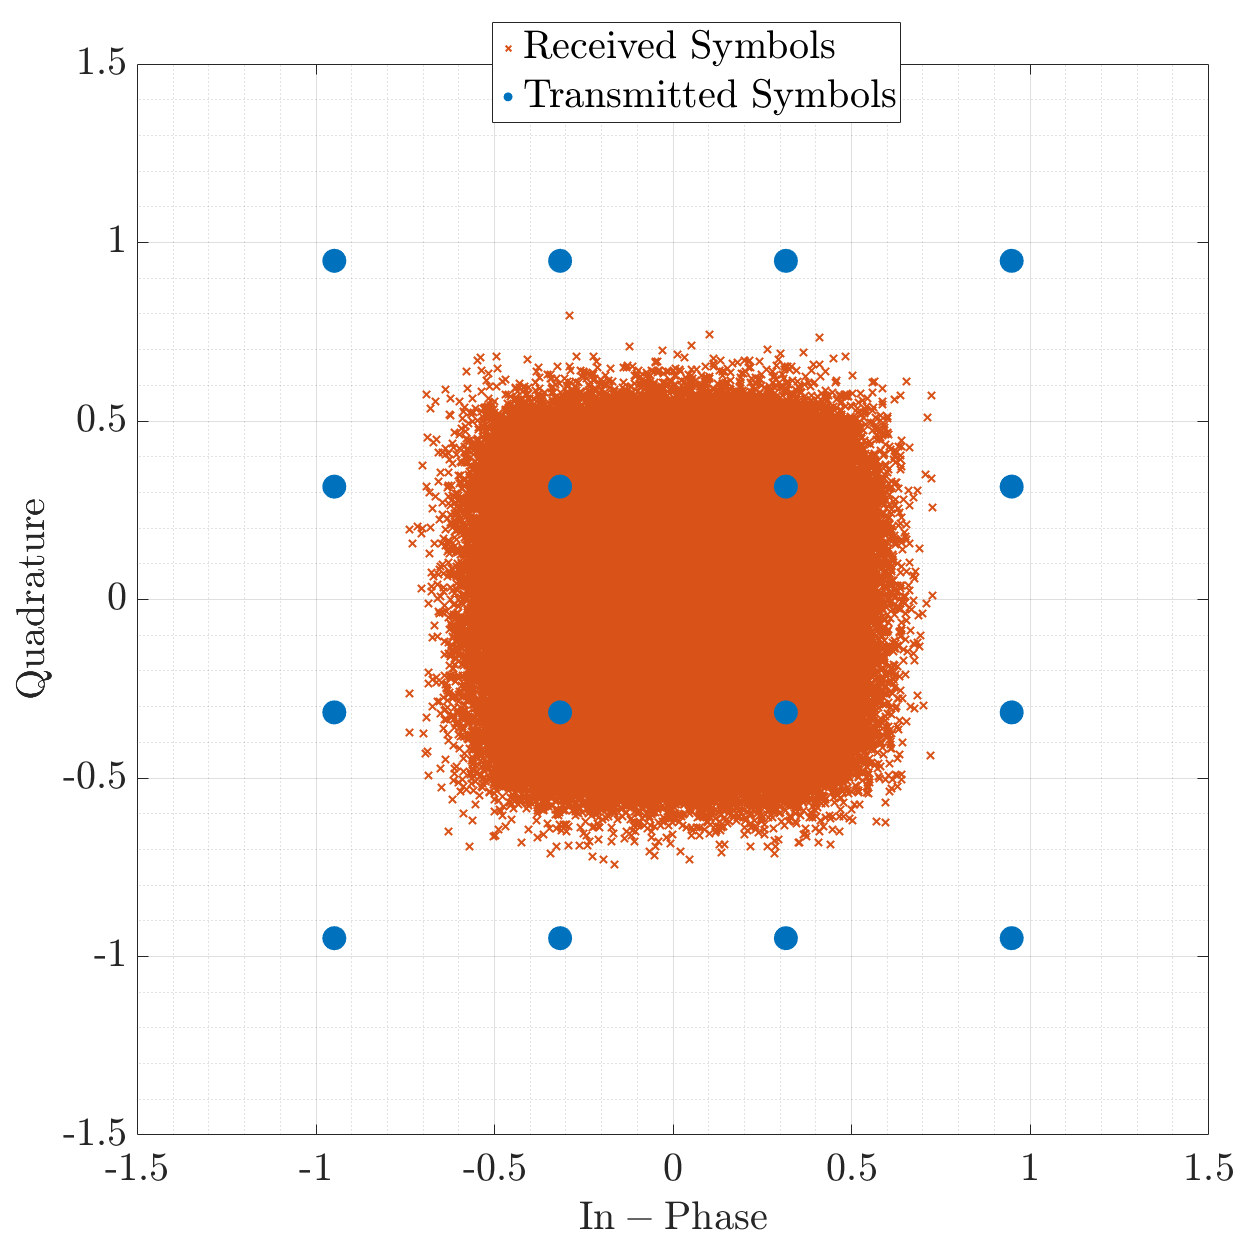
\includegraphics[width=\linewidth]{Images/const-noisy.png}
			\caption{Noisy 16-QAM before matched filtering.}
			\label{fig:const-noisy_cont_compact}
		\end{subfigure}\hfill
		\begin{subfigure}{0.4\textwidth}
			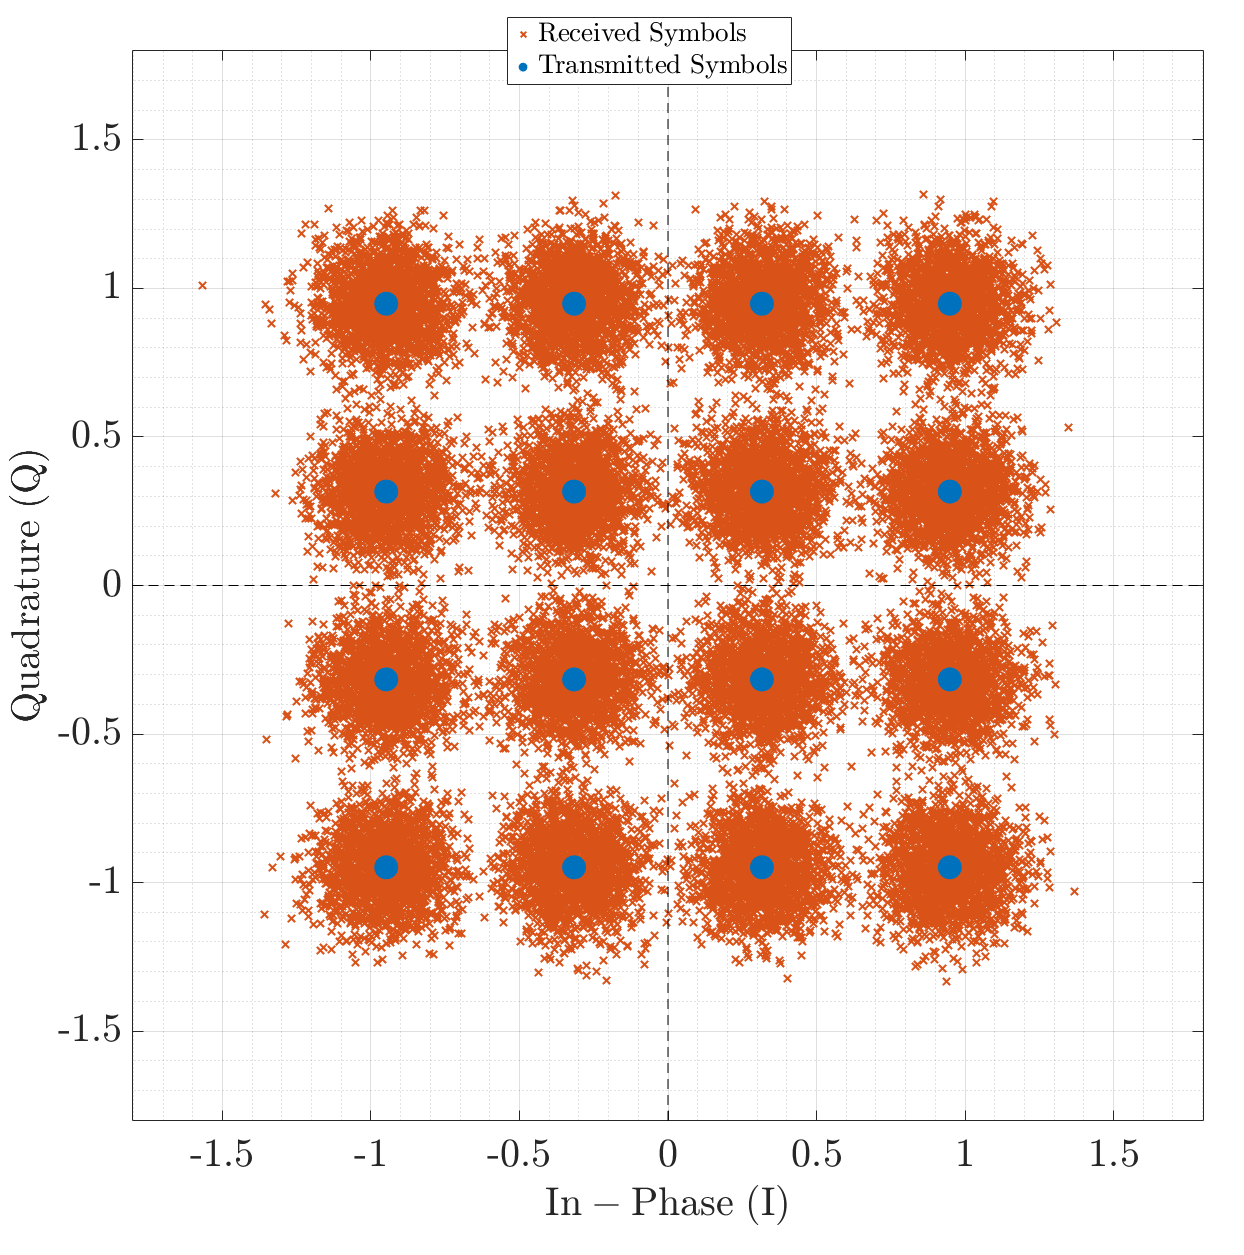
\includegraphics[width=\linewidth]{Images/const-filtered-down.png} 
			\caption{16-QAM after matched filtering.}
			\label{fig:const-filtered-down_cont_compact}
		\end{subfigure}
		\caption{Effect of AWGN and matched filtering on 16-QAM ($\frac{E_b}{N_0} = 15 \text{ dB}$).}
		\label{fig:constellations-noise_cont}
	\end{figure}
	
	\subsection{Questions: Optimal Communication Chain}
	\par\noindent\textbf{It is proposed to use the baseband equivalent model of the AWGN channel. Would it be possible to work with a bandpass implementation of the system? :}\quad\ignorespaces 
		Working with baseband equivalent models reduces complexity by avoiding high carrier frequencies, allowing lower simulation sampling rates and modular design of modulation/demodulation stages.
	\par
	
	\par\noindent\textbf{How do you choose the sample rate in Matlab? :}\quad\ignorespaces 
		The Matlab sampling rate $F_s$ must be at least twice the maximum signal frequency $F_{\text{max}}$ (Nyquist criterion) to prevent aliasing. For an RRC filter with roll-off $\beta$, the maximum frequency is
		\begin{equation} F_{\text{max}} = \frac{1+\beta}{2T_{\text{symb}}} \end{equation}
		Thus, the oversampling factor $M$ must ensure
		\begin{equation} F_s = M/T_{\text{symb}} \ge 2 F_{\text{max}} \end{equation}
	\par
	
	\par\noindent\textbf{How do you make sure you simulate the desired $E_b/N_0$ ratio? :}\quad\ignorespaces 
		Noise power is 
		\begin{equation} P_n = N_0 F_s \end{equation}
		$N_0$ is derived from the target $E_b/N_0$ and calculated bit energy $E_b$. $E_b$ is given by
		\begin{equation} E_b = \frac{E_s}{\log_2(M)} \end{equation}
		where $E_s$ is average symbol energy. Complex noise $n(t)$ is generated as
		\begin{equation} n(t) = \sqrt{\frac{P_n}{2}}(X+jY) \end{equation}
		with 
		\begin{equation} X, Y \sim \mathcal{N}(0,1) \end{equation}
	\par
	
	\par\noindent\textbf{How do you choose the number of transmitted data packets and their length? :}\quad\ignorespaces 
		The number of bits per packet must be a multiple of $\log_2(M)$ for M-QAM to avoid unused bits. Total transmitted bits must be sufficient for statistically relevant BER estimation, typically such that at least 10-100 errors are observed for the target BER.
	\par
			
	\par\noindent\textbf{Determine the supported (uncoded) bit rate as a function of the physical bandwidth? :}\quad\ignorespaces 
		The two-sided Nyquist bandwidth is
		\begin{equation} B = \frac{1+\beta}{T_{\text{symb}}} \end{equation}
		The bit rate $R_b$ is
		\begin{equation} R_b = \frac{\log_2 M}{T_{\text{symb}}} = (\log_2 M) \cdot R_{\text{symb}} \end{equation}
		Thus,
		\begin{equation} R_b = R_{\text{symb}} \cdot \log_2 M = \frac{B}{1+\beta} \log_2 M \end{equation}
	\par
			
	\par\noindent\textbf{Explain the trade-off communication capacity/reliability achieved by varying the constellation size? :}\quad\ignorespaces 
		Larger constellations (higher M) increase capacity (more bits/symbol, higher $R_b$ for fixed bandwidth). However, constellation points are closer, reducing Euclidean distance and increasing susceptibility to noise, thus degrading BER for a given $E_b/N_0$ (lower reliability).
	\par
			
	\par\noindent\textbf{Why do we choose the halfroot Nyquist filter to shape the complex symbols? :}\quad\ignorespaces 
		RRC filters are used because: 1) When paired (transmitter and matched receiver filter), they form an overall Nyquist filter, ensuring zero ISI at correct sampling instants. 2) The matched filter maximizes SNR at the detector input. 3) They provide good spectral containment.
	\par
			
	\par\noindent\textbf{How do we implement the optimal demodulator? Give the optimisation criterion? :}\quad\ignorespaces 
		The optimal demodulator for AWGN channels uses a filter matched to the transmitted pulse shape $g(t)$, i.e., $g^*(-t)$, followed by sampling at symbol instants $kT_{\text{symb}}$. This maximizes the output SNR.
	\par
			
	\par\noindent\textbf{How do we implement the optimal detector? Give the optimisation criterion? :}\quad\ignorespaces 
		The optimal detector minimizes symbol error probability. For equiprobable symbols in AWGN, this corresponds to the Maximum Likelihood (ML) criterion: choose symbol $s_m$ that maximizes $p(r|s_m)$. This simplifies to minimizing the Euclidean distance:
		\begin{equation} \hat{s}_{\text{ML}} = \operatorname*{arg\,min}_{s_m} ||r - s_m||^2 \end{equation}
	\par
			
	\section{Time and Frequency Synchronization}
	Synchronization aims to align the receiver's timing and carrier frequency with those of the transmitter. Errors include Carrier Frequency Offset ($\Delta f$), Phase Offset ($\phi_0$), and Sample Time Shift ($t_0$), illustrated in Figure \ref{fig:sync-errors-conceptual}.
			
	\begin{figure}[H]
		\centering
		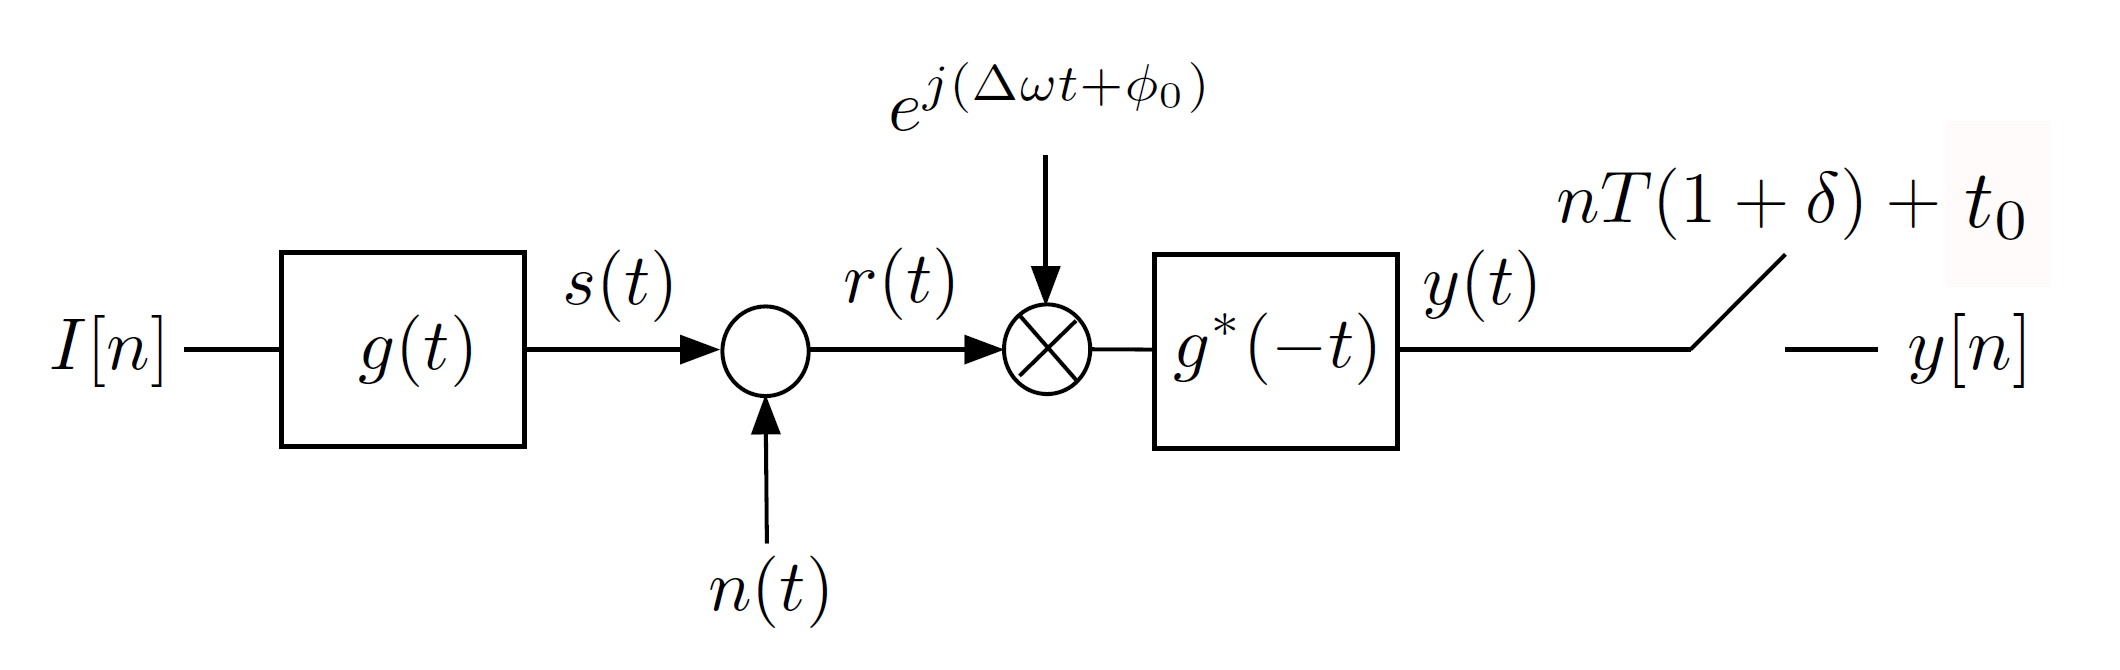
\includegraphics[width=0.6\linewidth]{Images/sync-errors-conceptual} 
		\caption{Synchronization mismatches.}
		\label{fig:sync-errors-conceptual}
	\end{figure}
	
	\subsection{Impact Assessment of CFO and Carrier Phase Error}
	Synchronization errors degrade performance. A Phase Offset ($\phi_0$) rotates the received constellation, meaning $y[n] = I[n]e^{j\phi_0}$, whereas a Carrier Frequency Offset ($\Delta f$) causes a progressive phase drift and can also lead to ISI due to mismatch with the receiver's filter. 
	\begin{equation} y[n] = I[n]e^{j(2\pi \Delta f nT_{\text{symb}} + \phi_0')} \end{equation}
	
	
	\subsection{Impact Assessment of Sample Time Shift}
	A Sample Time Shift ($t_0$) also degrades performance by causing signal attenuation and ISI, as described by:
	\begin{equation} y[n] = I[n]h(t_0) + \sum_{m \neq n} I[m]h((n-m)T_{\text{symb}} + t_0) \end{equation}
	
	Figures \ref{fig:ber_sync_errors} and \ref{fig:const_sync_errors} show these impacts on BER and 16-QAM constellations.
				
	\begin{figure}[H]
		\centering
		\begin{subfigure}[b]{0.48\textwidth}
			\centering
			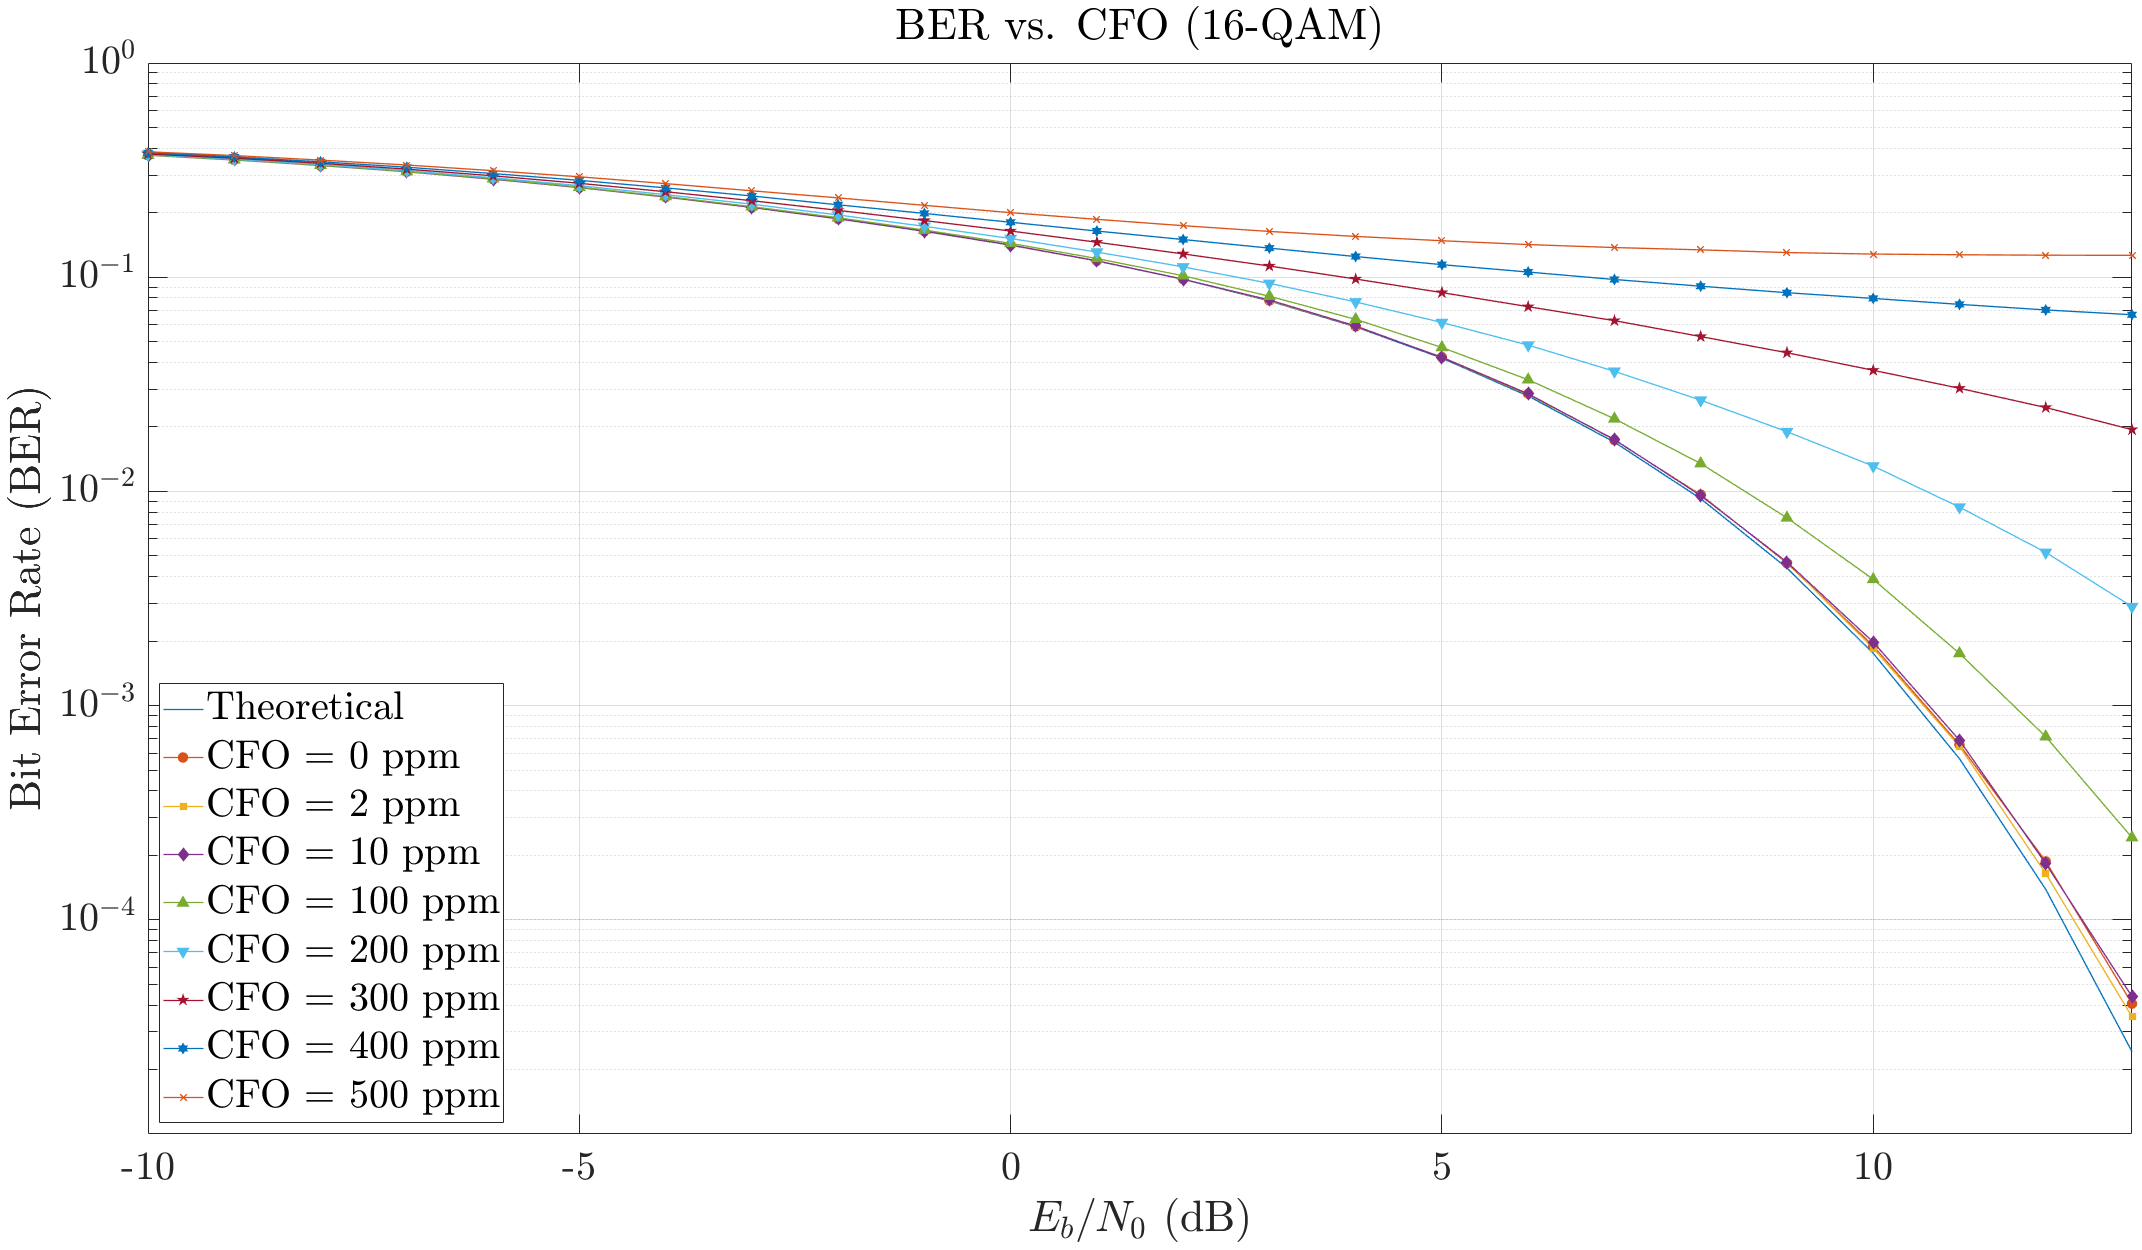
\includegraphics[width=\linewidth]{Images/ber-cfo}
			\caption{BER vs. $E_b/N_0$ for varying CFO.}
			\label{fig:ber-cfo_compact}
		\end{subfigure}
		\hfill
		\begin{subfigure}[b]{0.48\textwidth}
			\centering
			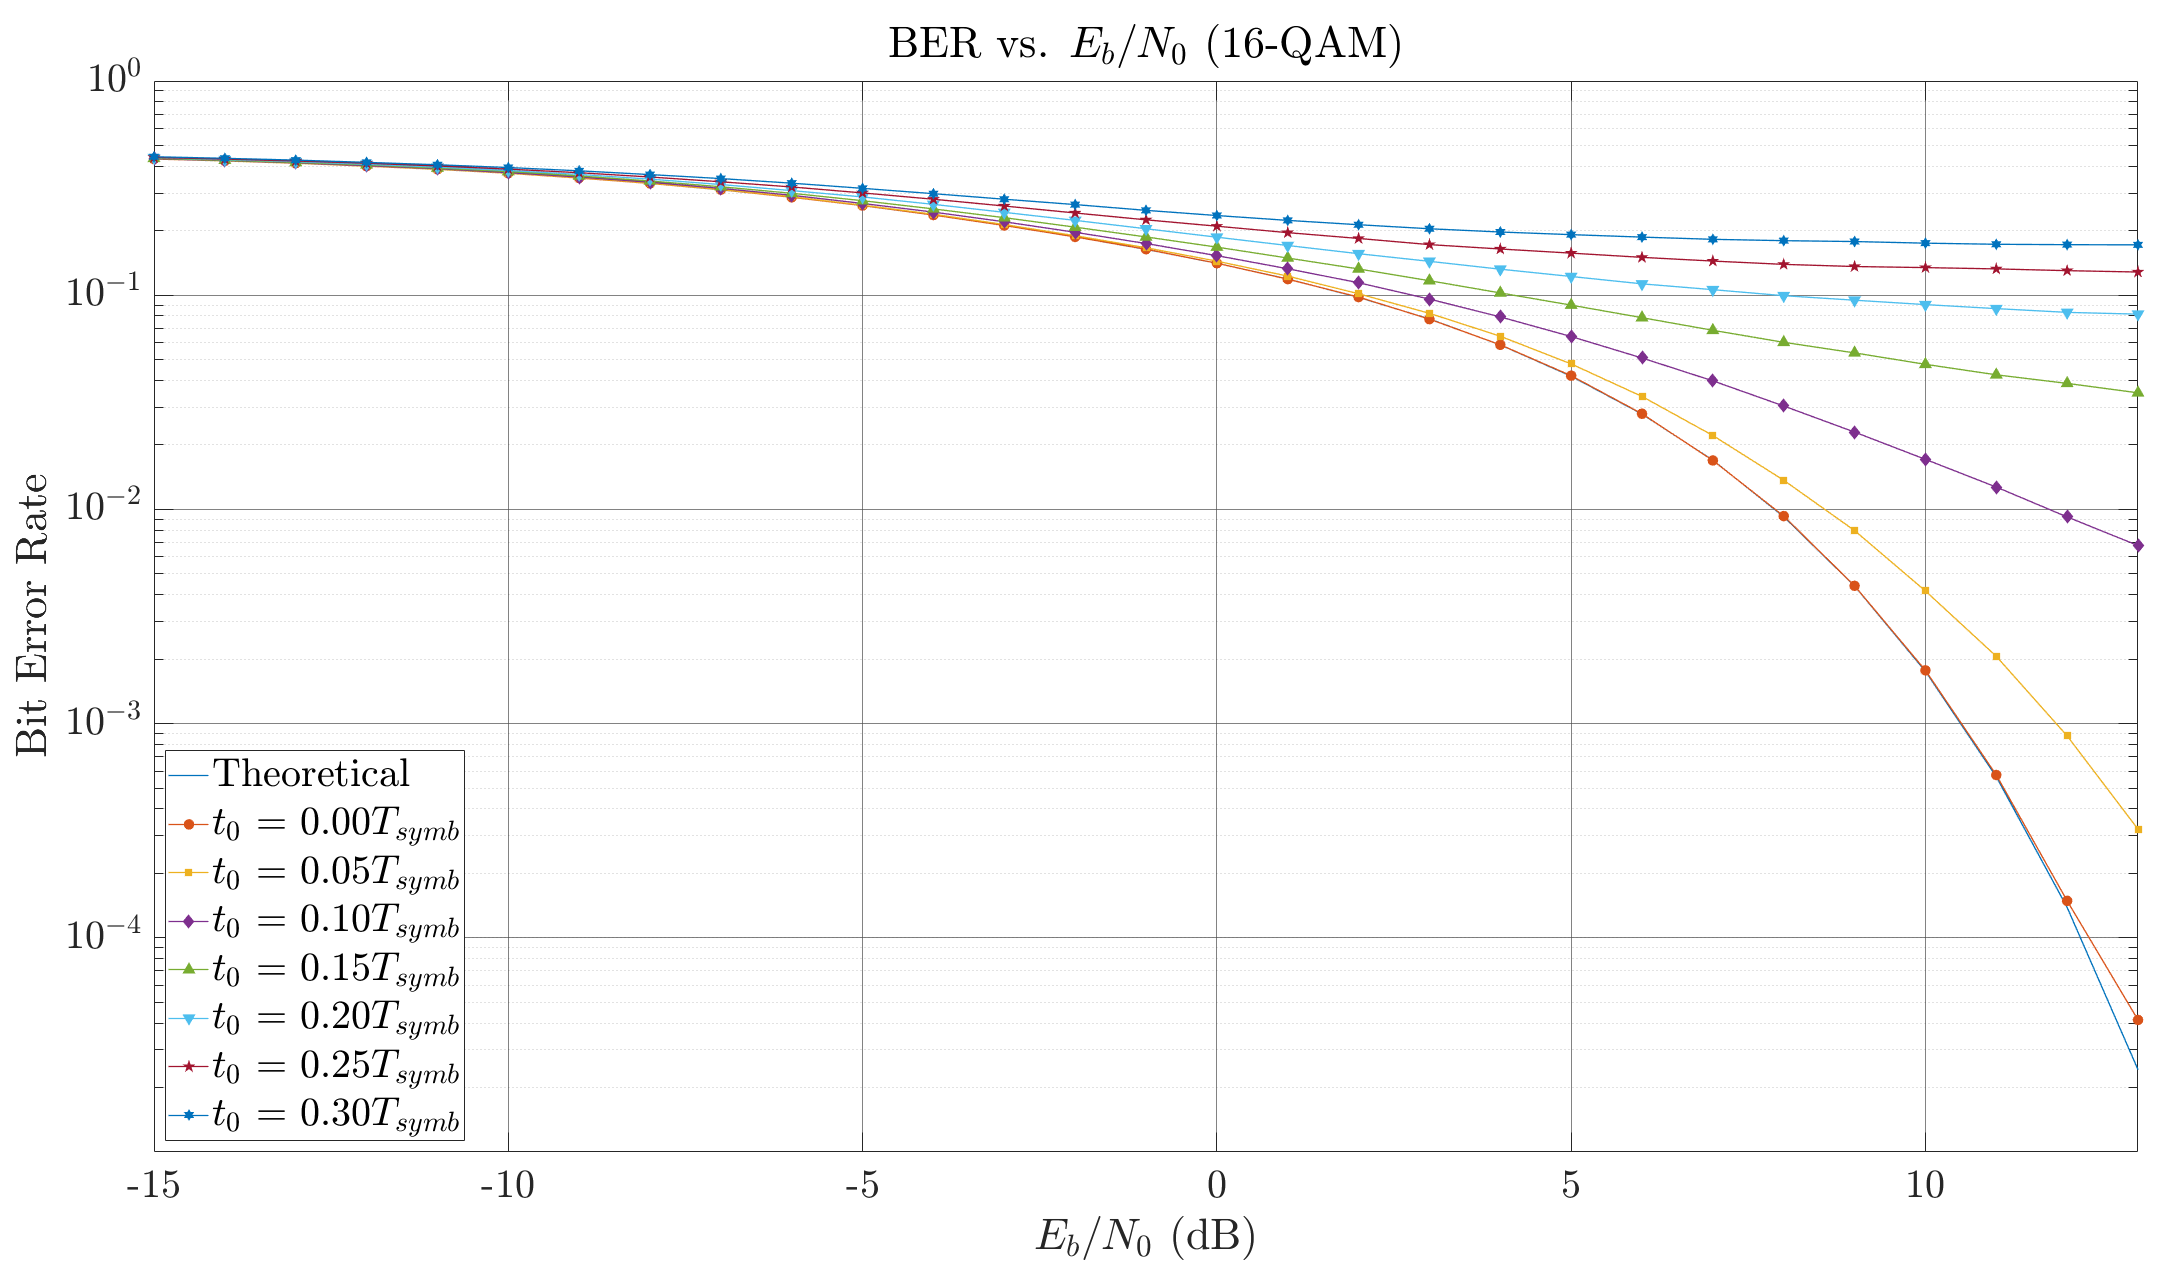
\includegraphics[width=\linewidth]{Images/ber-timing}
			\caption{BER vs. $E_b/N_0$ for varying $t_0/T_{\text{symb}}$.}
			\label{fig:ber-timing_compact}
		\end{subfigure}
		\caption{Impact of CFO and timing errors on BER for 16-QAM.}
		\label{fig:ber_sync_errors}
	\end{figure}
			
	\begin{figure}[H]
		\centering
		\begin{subfigure}[t]{0.4\textwidth}
			\centering
			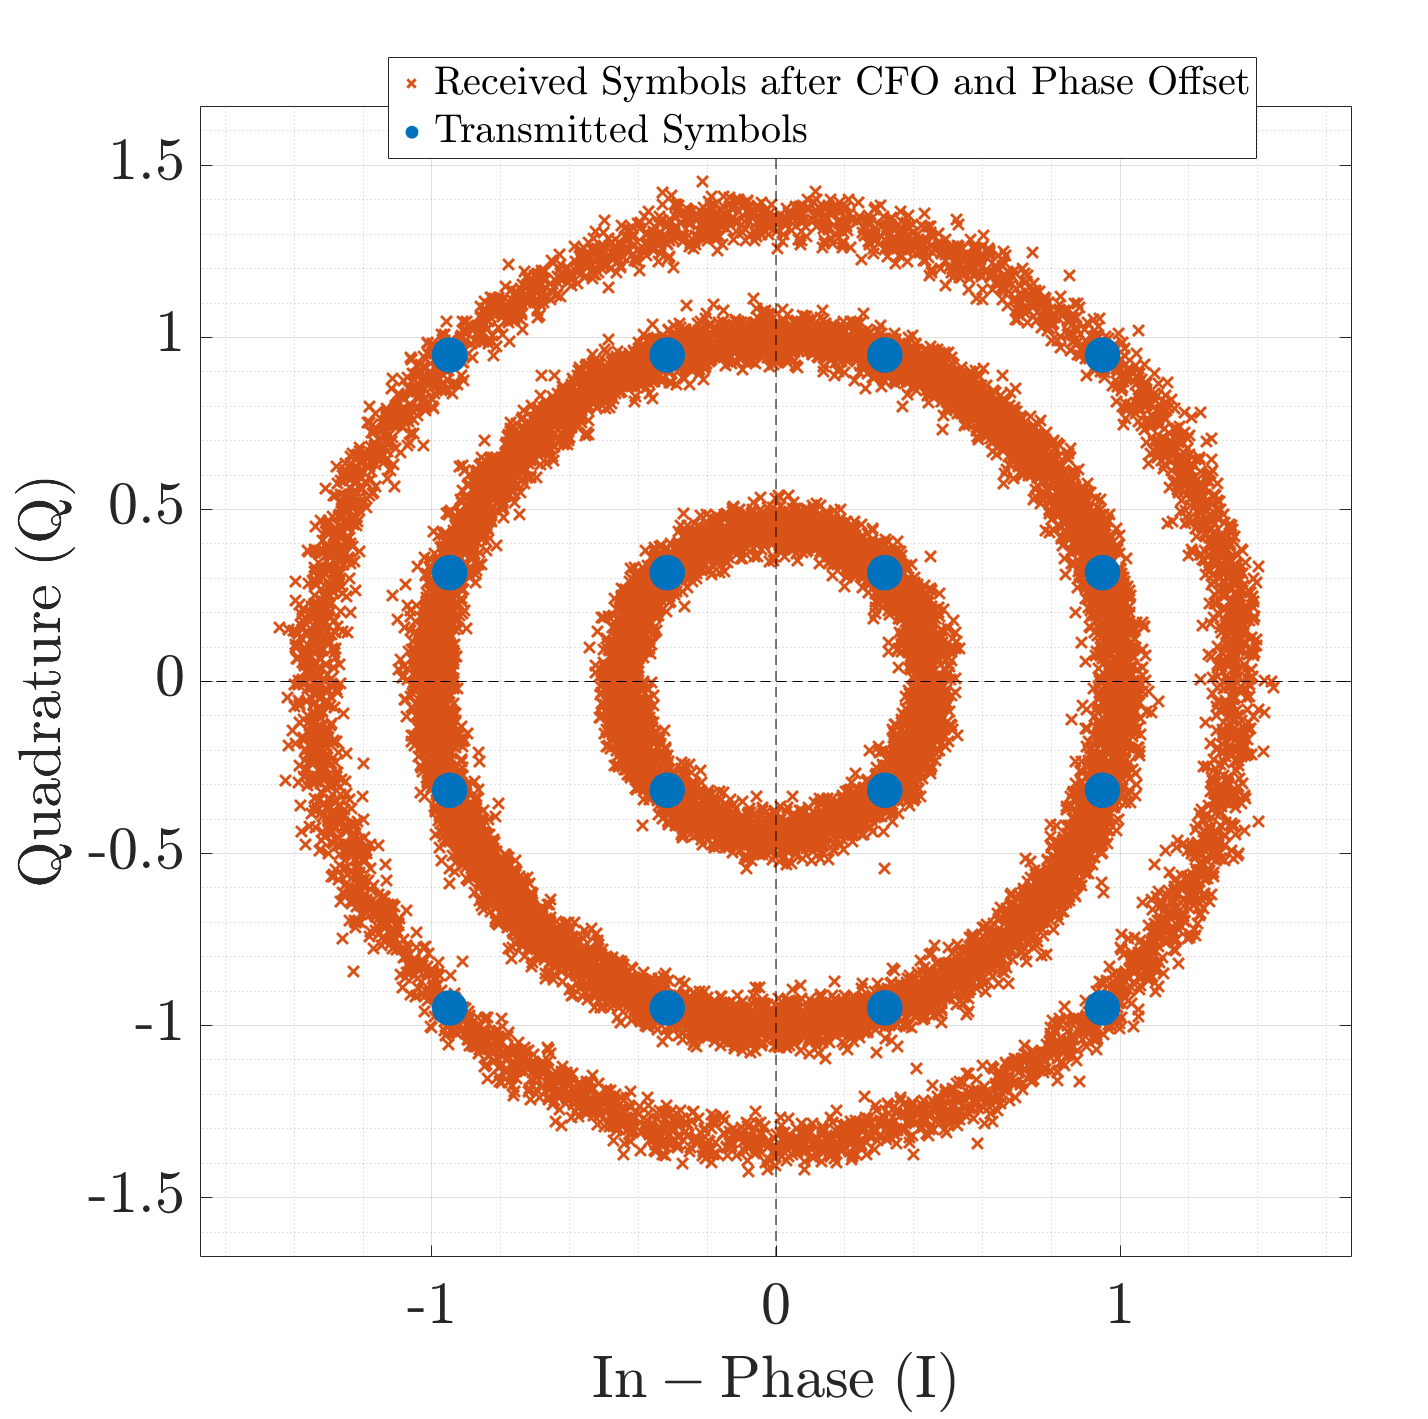
\includegraphics[width=\linewidth]{Images/cfo-po}
			\caption{Constellation with CFO and Phase Offset.}
			\label{fig:cfo-po-sub_compact}
		\end{subfigure}
		\hfill
		\begin{subfigure}[t]{0.4\textwidth}
			\centering
			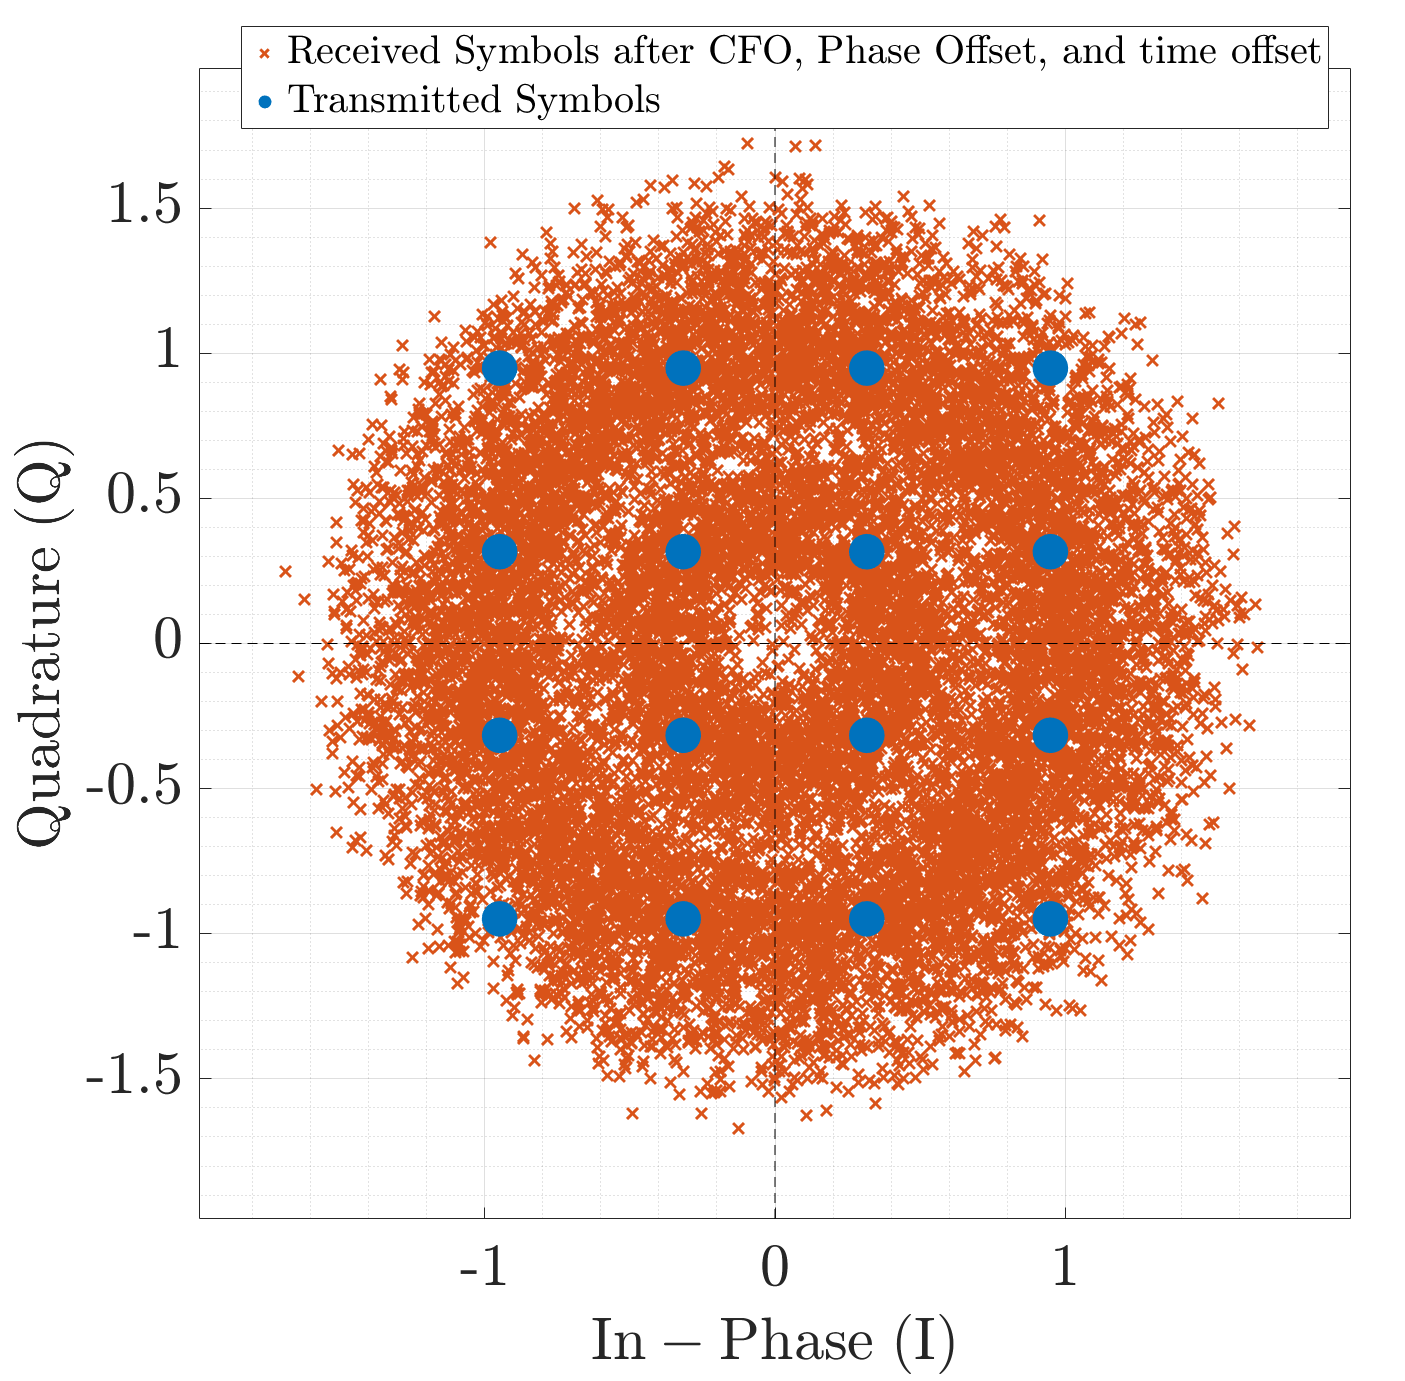
\includegraphics[width=\linewidth]{Images/cfo-po-to}
			\caption{Constellation with CFO, Phase Offset, and Time Offset.}
			\label{fig:cfo-po-to-sub_compact}
		\end{subfigure}
		\caption{Impact of synchronization errors on 16-QAM constellation ($E_b/N_0 = 20 \text{ dB}$).}
		\label{fig:const_sync_errors}
	\end{figure}
	
	\subsection{Gardner Algorithm Implementation}
	The Gardner algorithm is a Non data-aided (NDA) feedback loop that determine an  estimate $\hat{\epsilon}[n]$ of the sampling time errors $\epsilon[n]$, such that: 
	\begin{equation}
		\hat{\epsilon}[n+1] = \hat{\epsilon}[n] - \kappa \cdot \operatorname{Re} \left\{ y_{\hat{\epsilon}[n]}[n-1/2] \left( y_{\hat{\epsilon}[n]}^{*}[n] - y_{\hat{\epsilon}[n-1]}^{*}[n-1] \right) \right\}
	\end{equation}
	Figure \ref{fig:gardner_performance} (a) shows convergence for different loop gains $\kappa$, and (b) demonstrates robustness to CFO.
			
	\begin{figure}[H]
		\centering
		\begin{subfigure}[b]{0.48\textwidth}
			\centering
			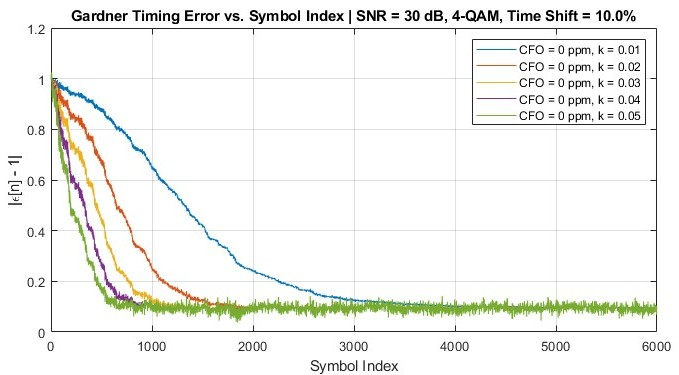
\includegraphics[width=\linewidth]{Images/Gardner_k_list.jpg} 
			\caption{Convergence for different $\kappa$.}
			\label{fig:gardner1_compact}
		\end{subfigure}
		\hfill
		\begin{subfigure}[b]{0.48\textwidth}
			\centering
			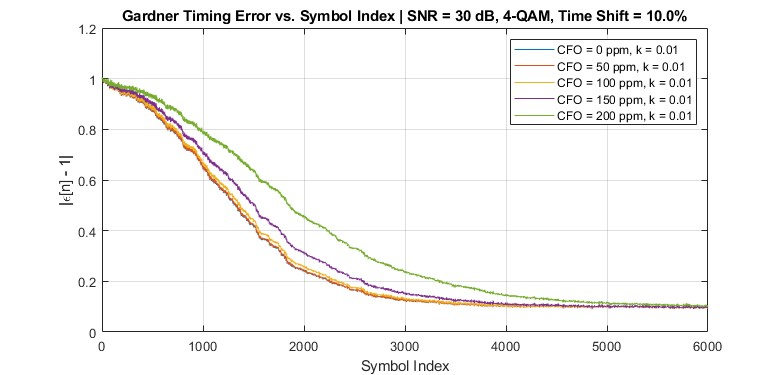
\includegraphics[width=\linewidth]{Images/Gardner_CFO_robust.jpg} 
			\caption{Robustness to CFO.}
			\label{fig:gardner2_compact}
		\end{subfigure}
		\caption{Gardner algorithm performance: time error convergence.}
		\label{fig:gardner_performance}
	\end{figure}
	
	\subsection{Frame and Frequency Acquisition Implementation}		
	Frame acquisition and coarse CFO estimation are performed using a data-aided (DA) differential cross-correlator. The differential cross-correlator $D_k[n]$ is computed from the known pilot sequence $a[l]$ as follows:
	\begin{equation}
		D_k[n] = \frac{1}{N-k} \sum_{l=k}^{N-1} (y^*[n+l]a[l])(y^*[n+l-k]a[l-k])^* \label{eq:diff_corr_metric_style_change}
	\end{equation}
	The pilot starting index $\hat{n}$, which is the Time of Arrival (ToA) of the pilot sequence is found by:
	\begin{equation} \hat{n} = \operatorname*{arg\,max}_n \sum_{k=1}^{K} |D_k[n]| \end{equation}
	The estimate of the CFO $\hat{\Delta f}$ is expressed as:
	\begin{equation} \hat{\Delta f} = -\frac{1}{K} \sum_{k=1}^{K} \frac{\angle D_k[\hat{n}]}{2\pi k T_{\text{symb}}} \end{equation}
	Figures \ref{fig:acquisition_vs_pilot_len_compact} and \ref{fig:acquisition_vs_K_avg_compact} show ToA and CFO estimation error standard deviations versus $E_b/N_0$ for varying pilot lengths $N$ and averaging windows $K$, respectively. As expected, longer pilot sequences and an optimized averaging window $K$  lead to improved estimation accuracy.
			
	\begin{figure}[H]
		\centering
		\begin{subfigure}[b]{0.4\textwidth}
			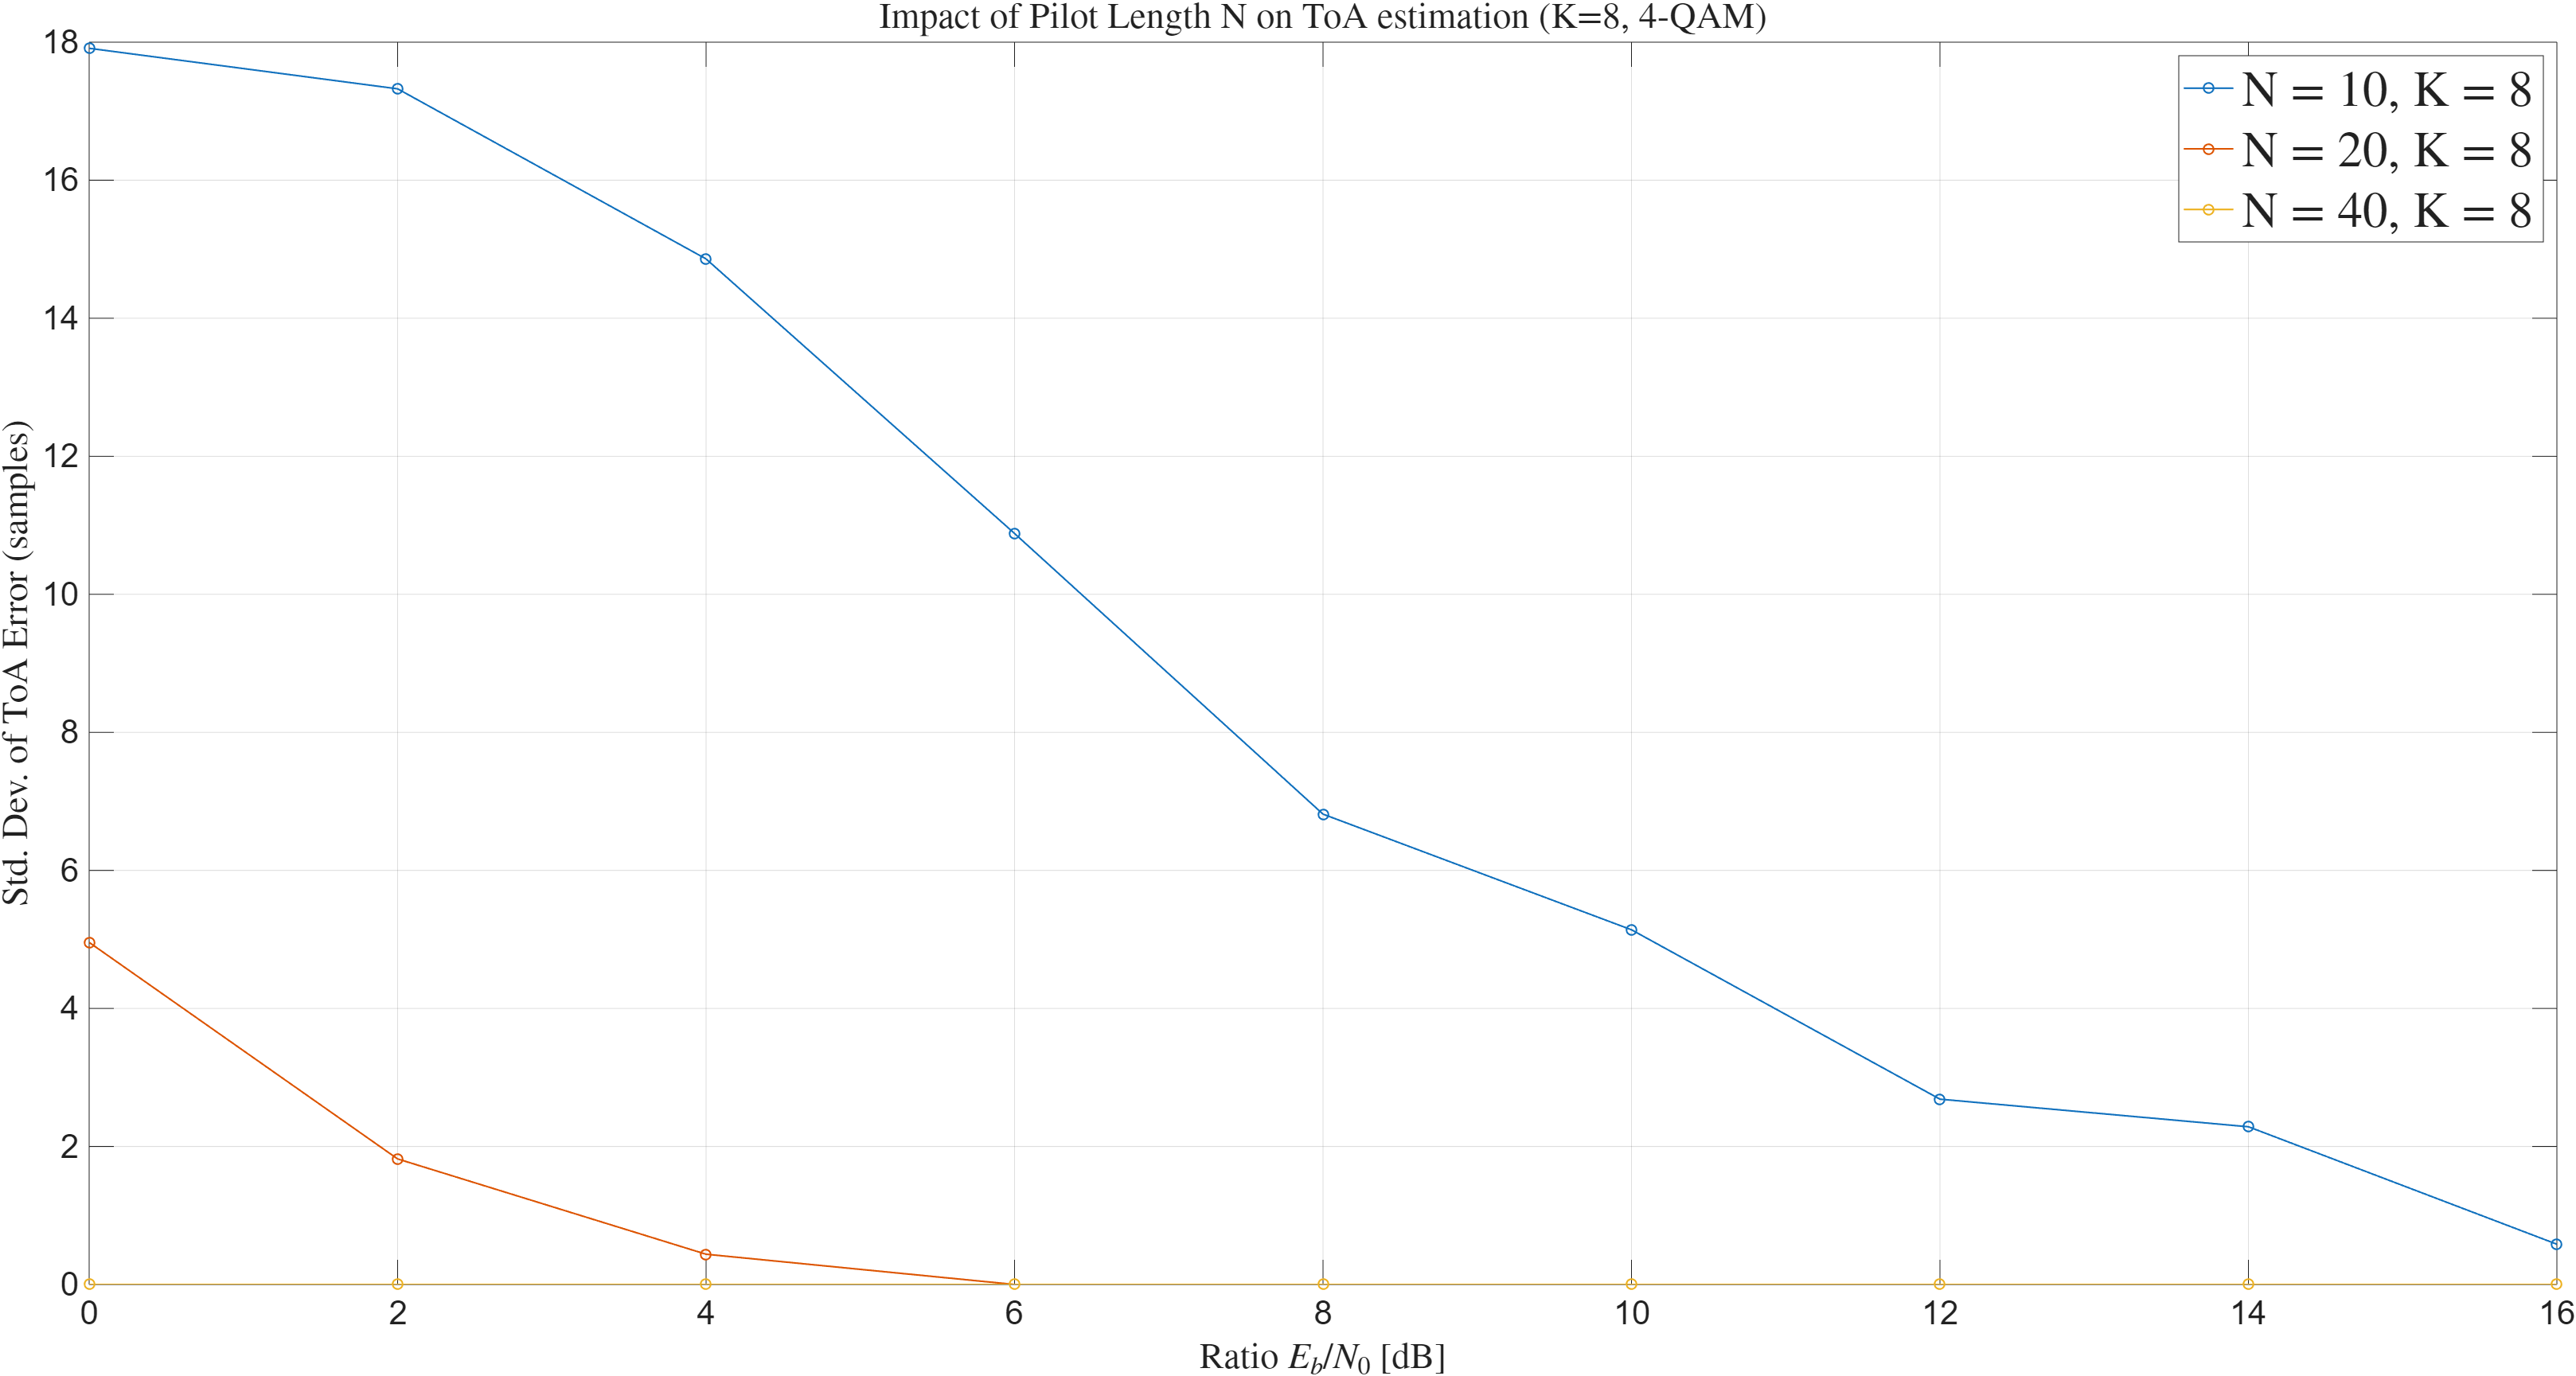
\includegraphics[width=\linewidth]{Images/frame_sync_pilot_len.png} 
			\caption{ToA error std dev vs. $N$}
		\end{subfigure}
		\hfill
		\begin{subfigure}[b]{0.4\textwidth}
			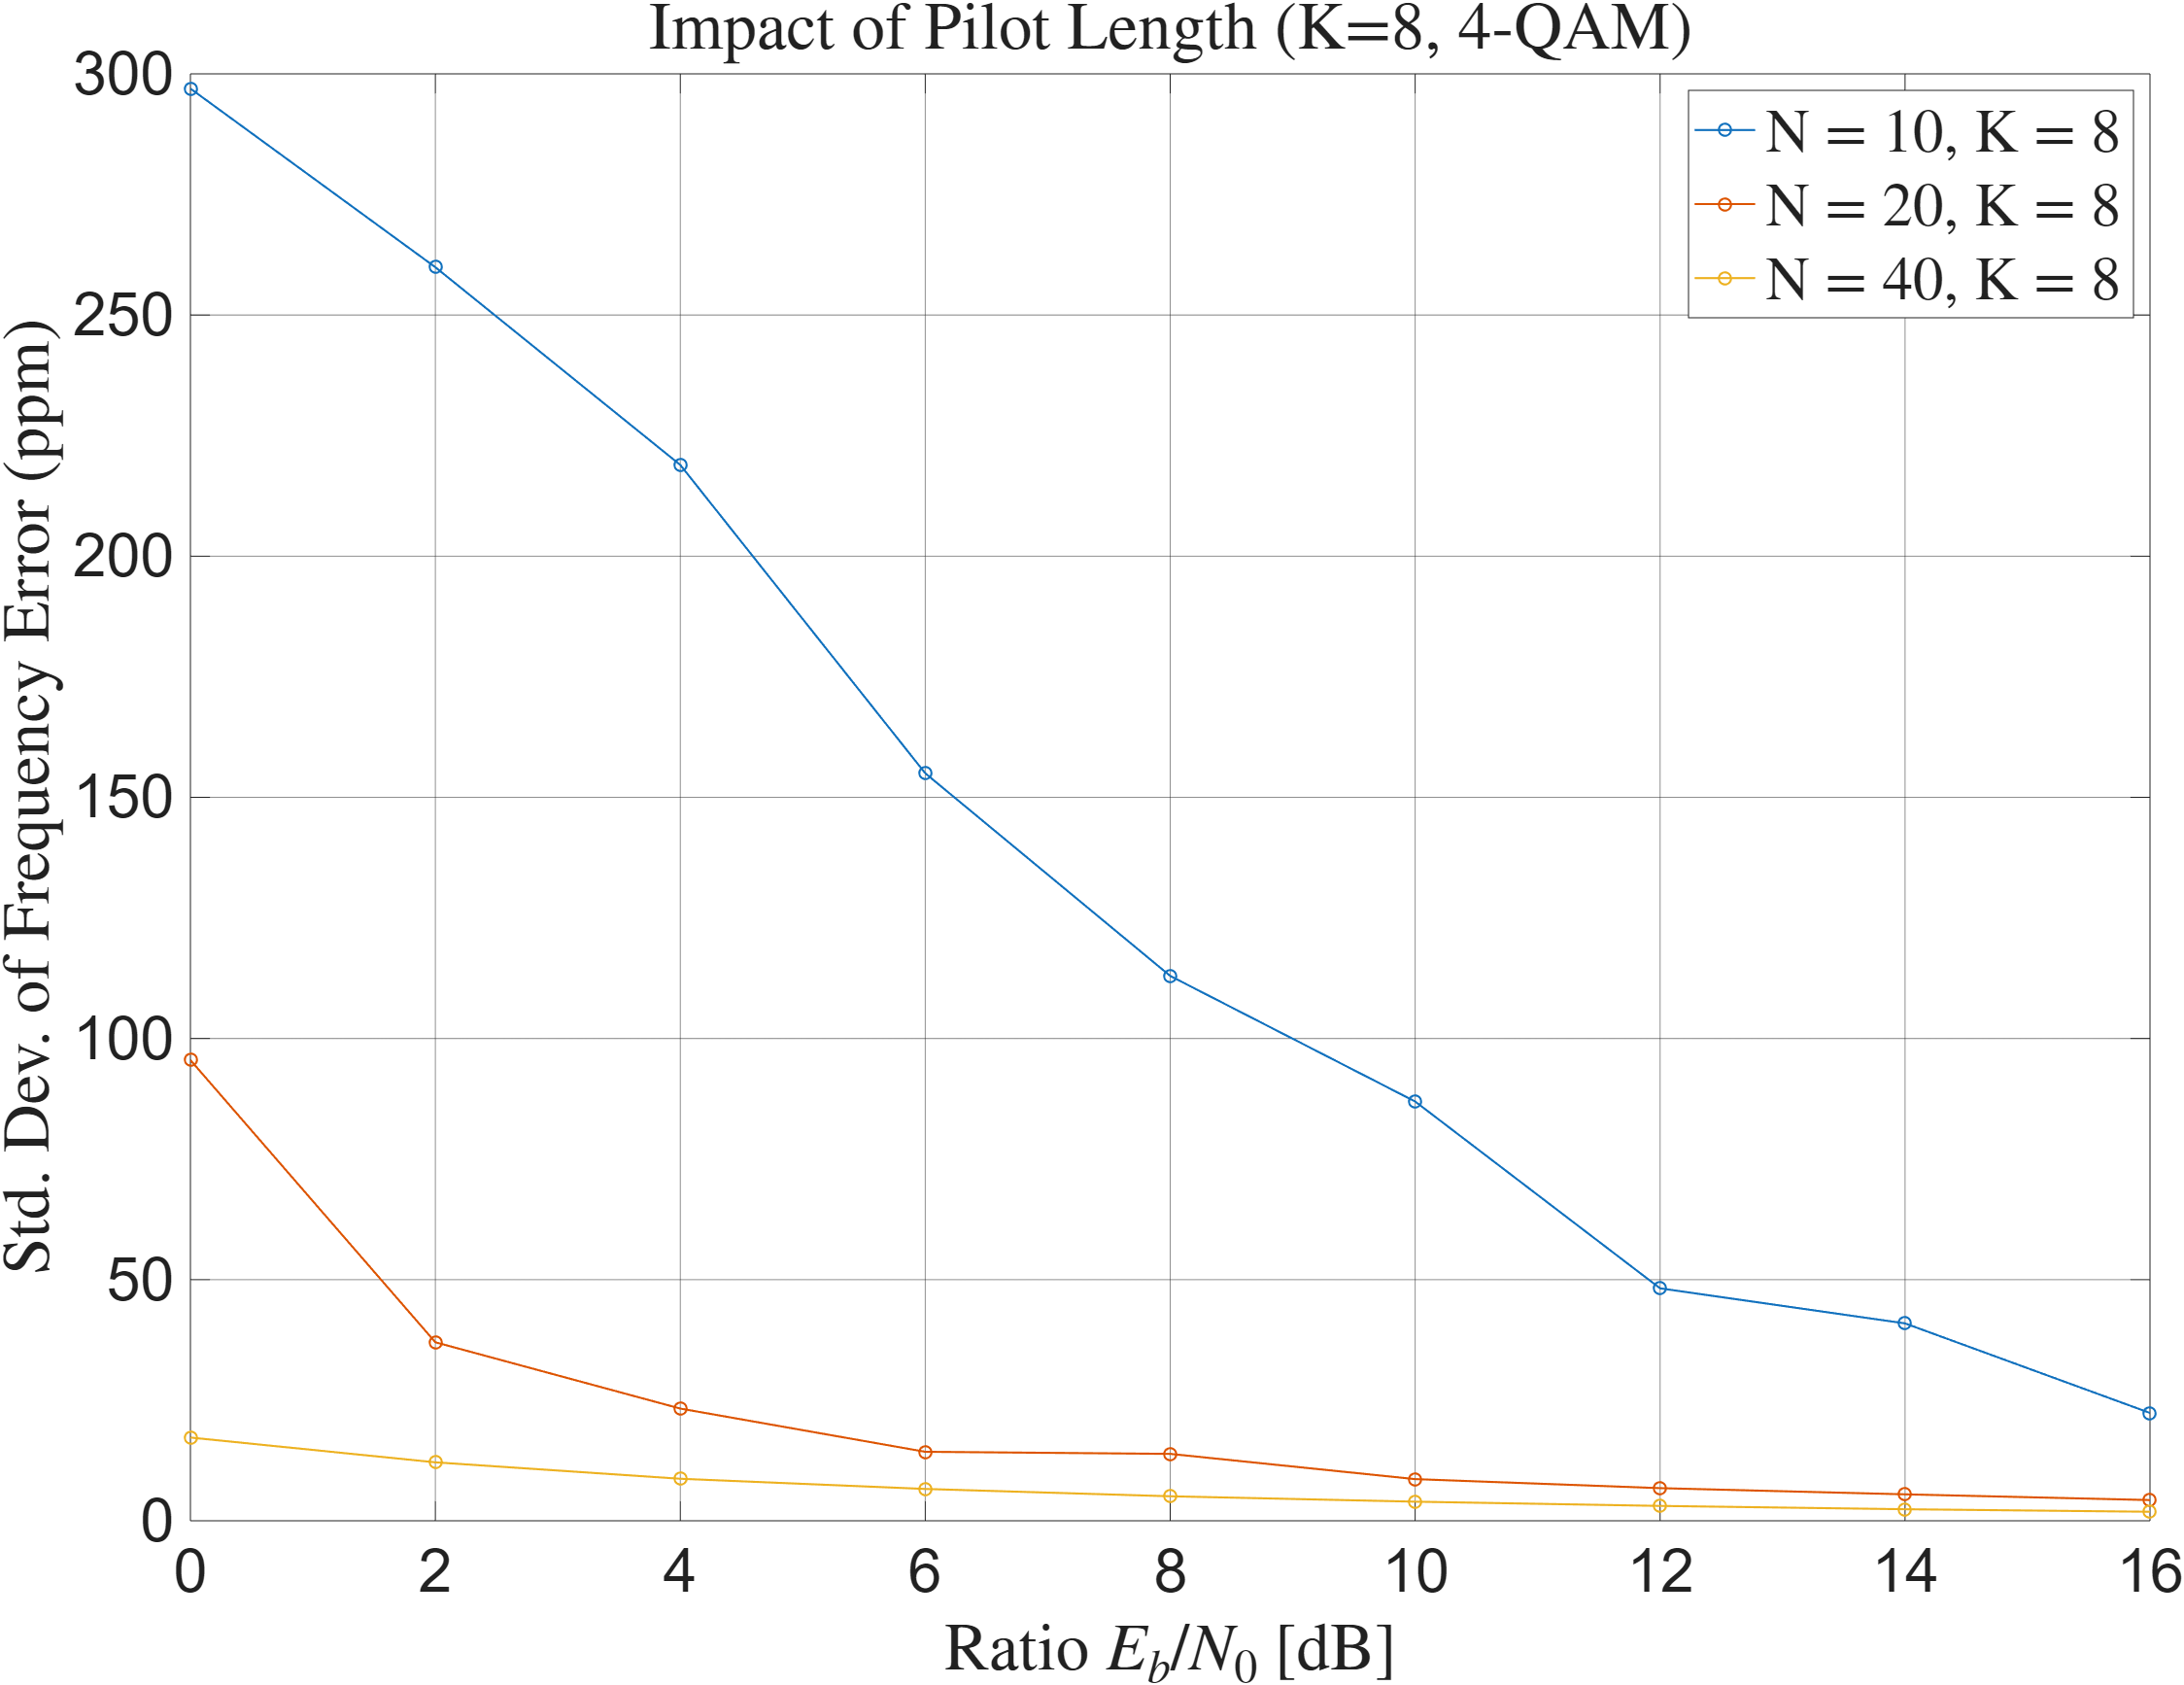
\includegraphics[width=\linewidth]{Images/cfo_est_pilot_len.png} 
			\caption{CFO error std dev vs. $N$}
		\end{subfigure}
		\caption{Acquisition error vs. $E_b/N_0$ for different pilot lengths ($N$).}
		\label{fig:acquisition_vs_pilot_len_compact}
	\end{figure}
			
	\begin{figure}[H]
		\centering
		\begin{subfigure}[b]{0.4\textwidth}
			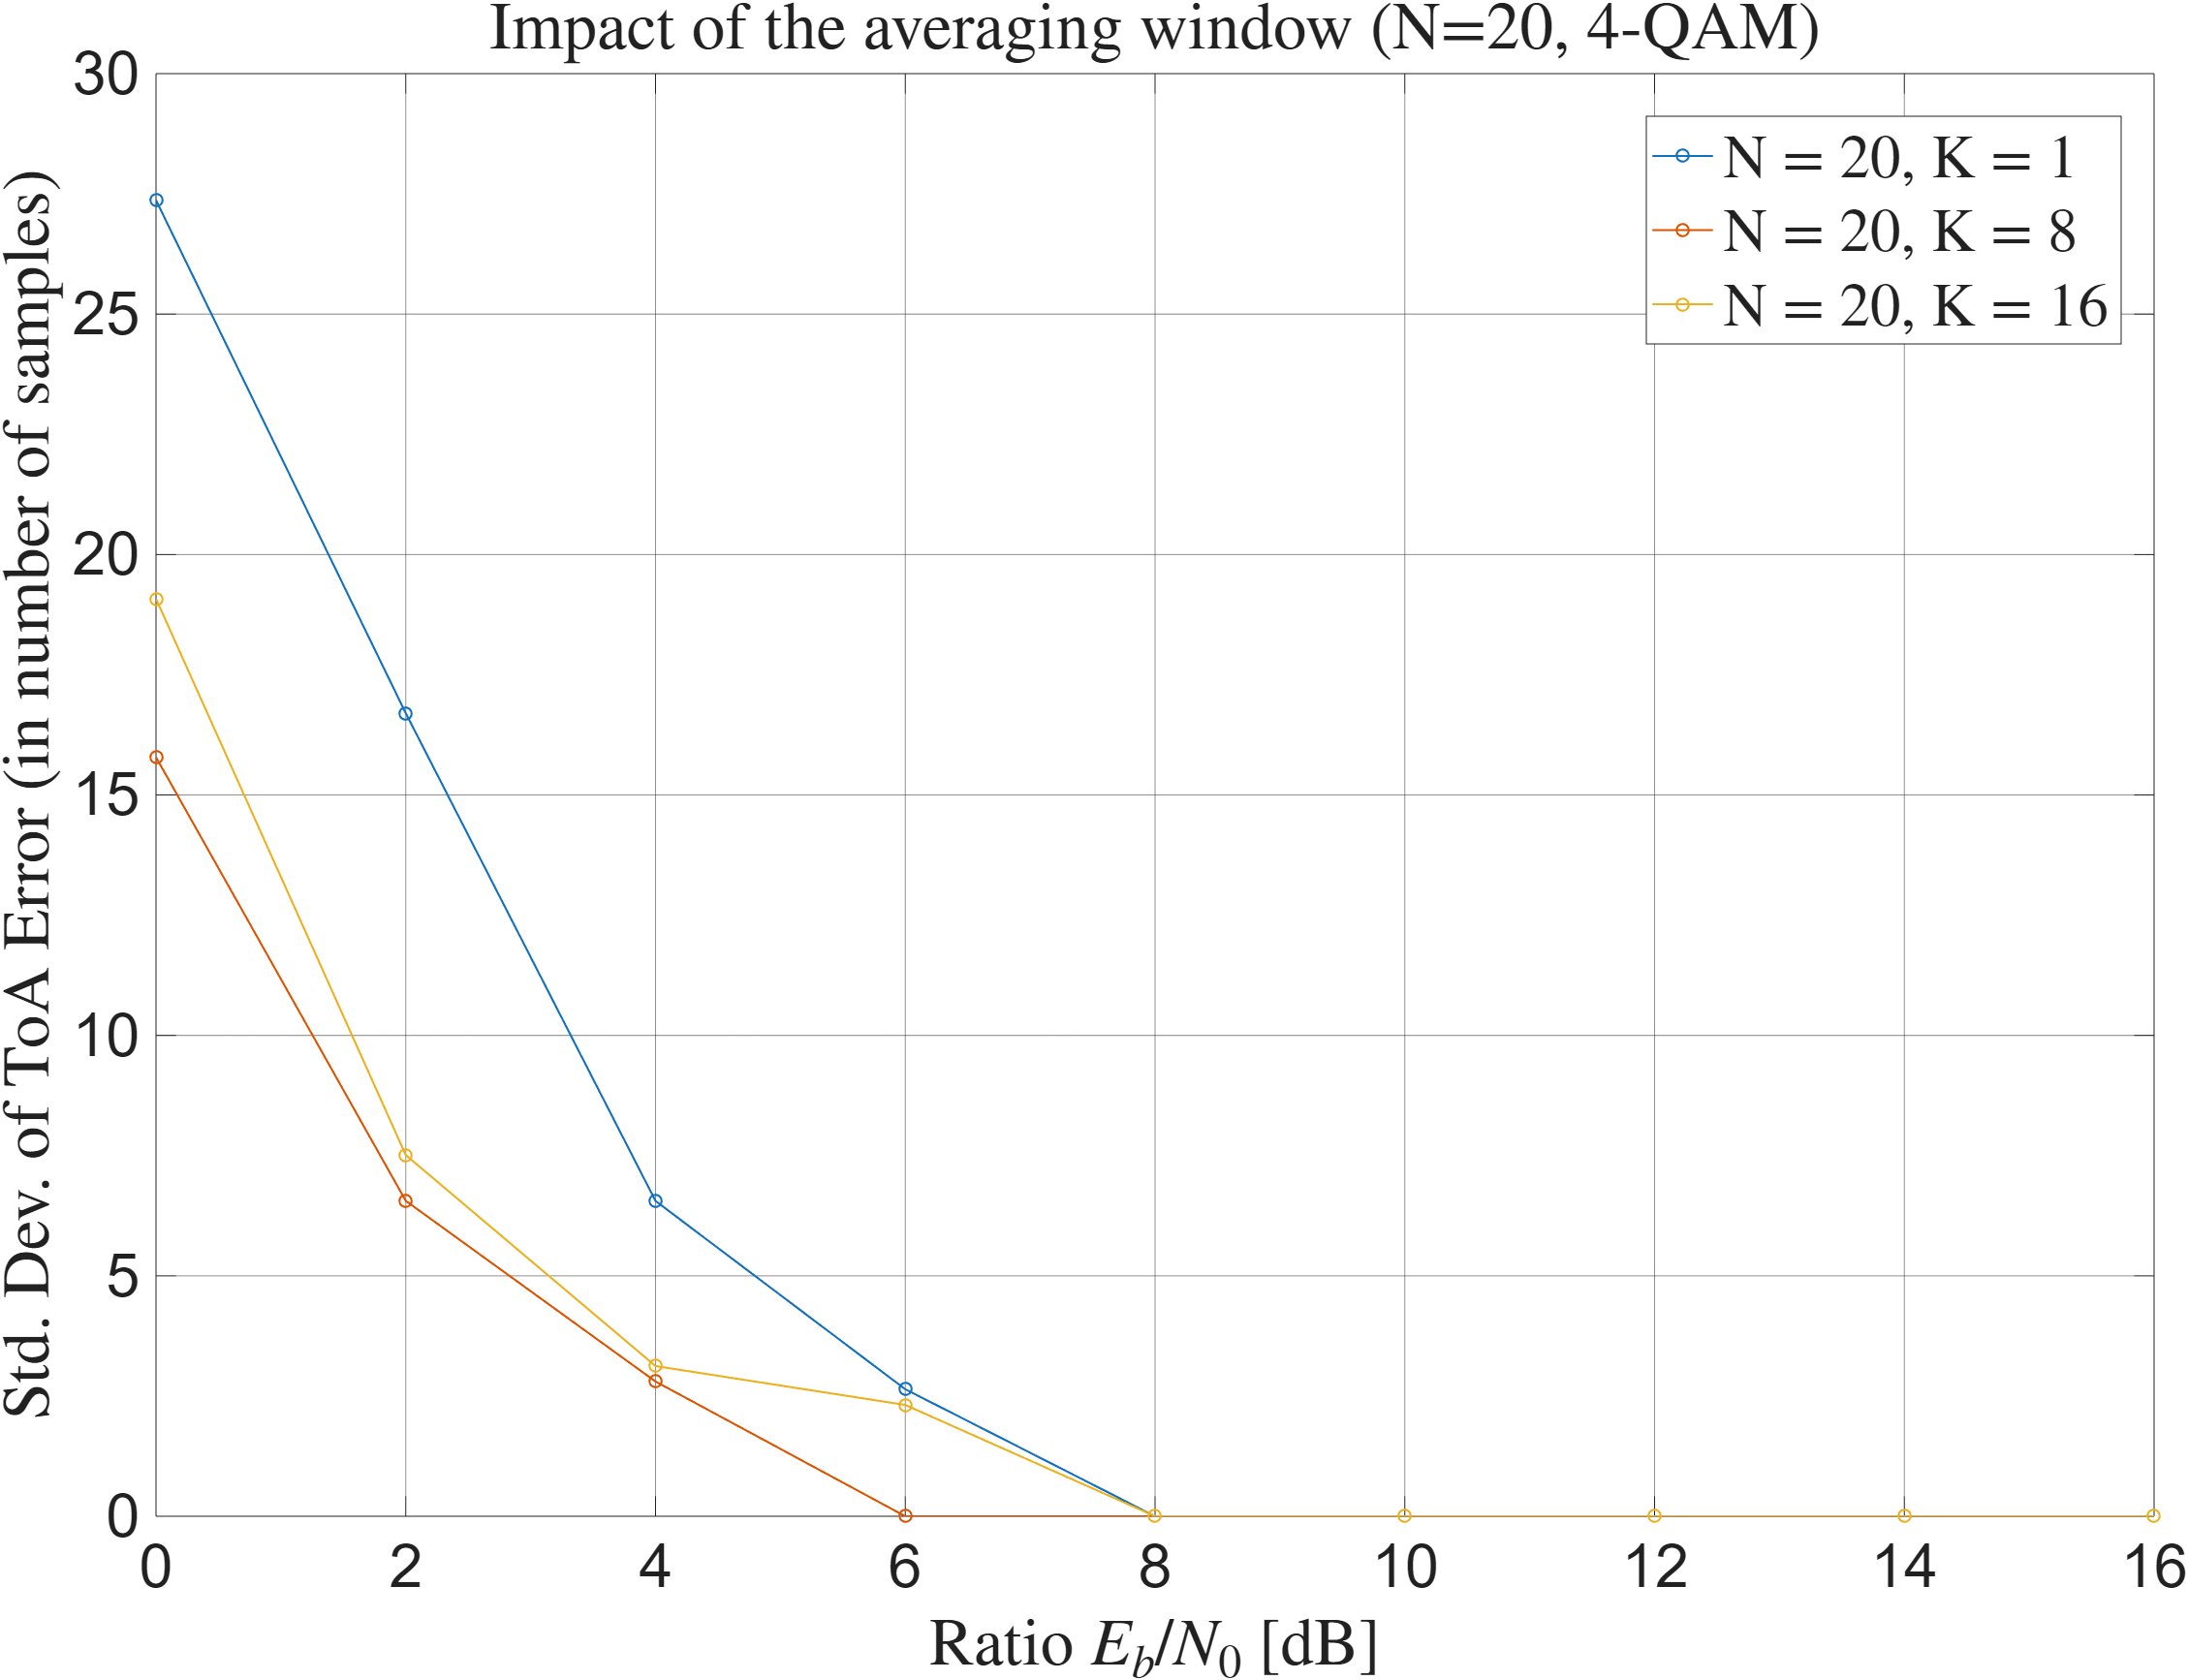
\includegraphics[width=\linewidth]{Images/frame_sync_K_avg.png} 
			\caption{ToA error std dev vs. $K$.}
		\end{subfigure}
		\hfill
		\begin{subfigure}[b]{0.4\textwidth}
			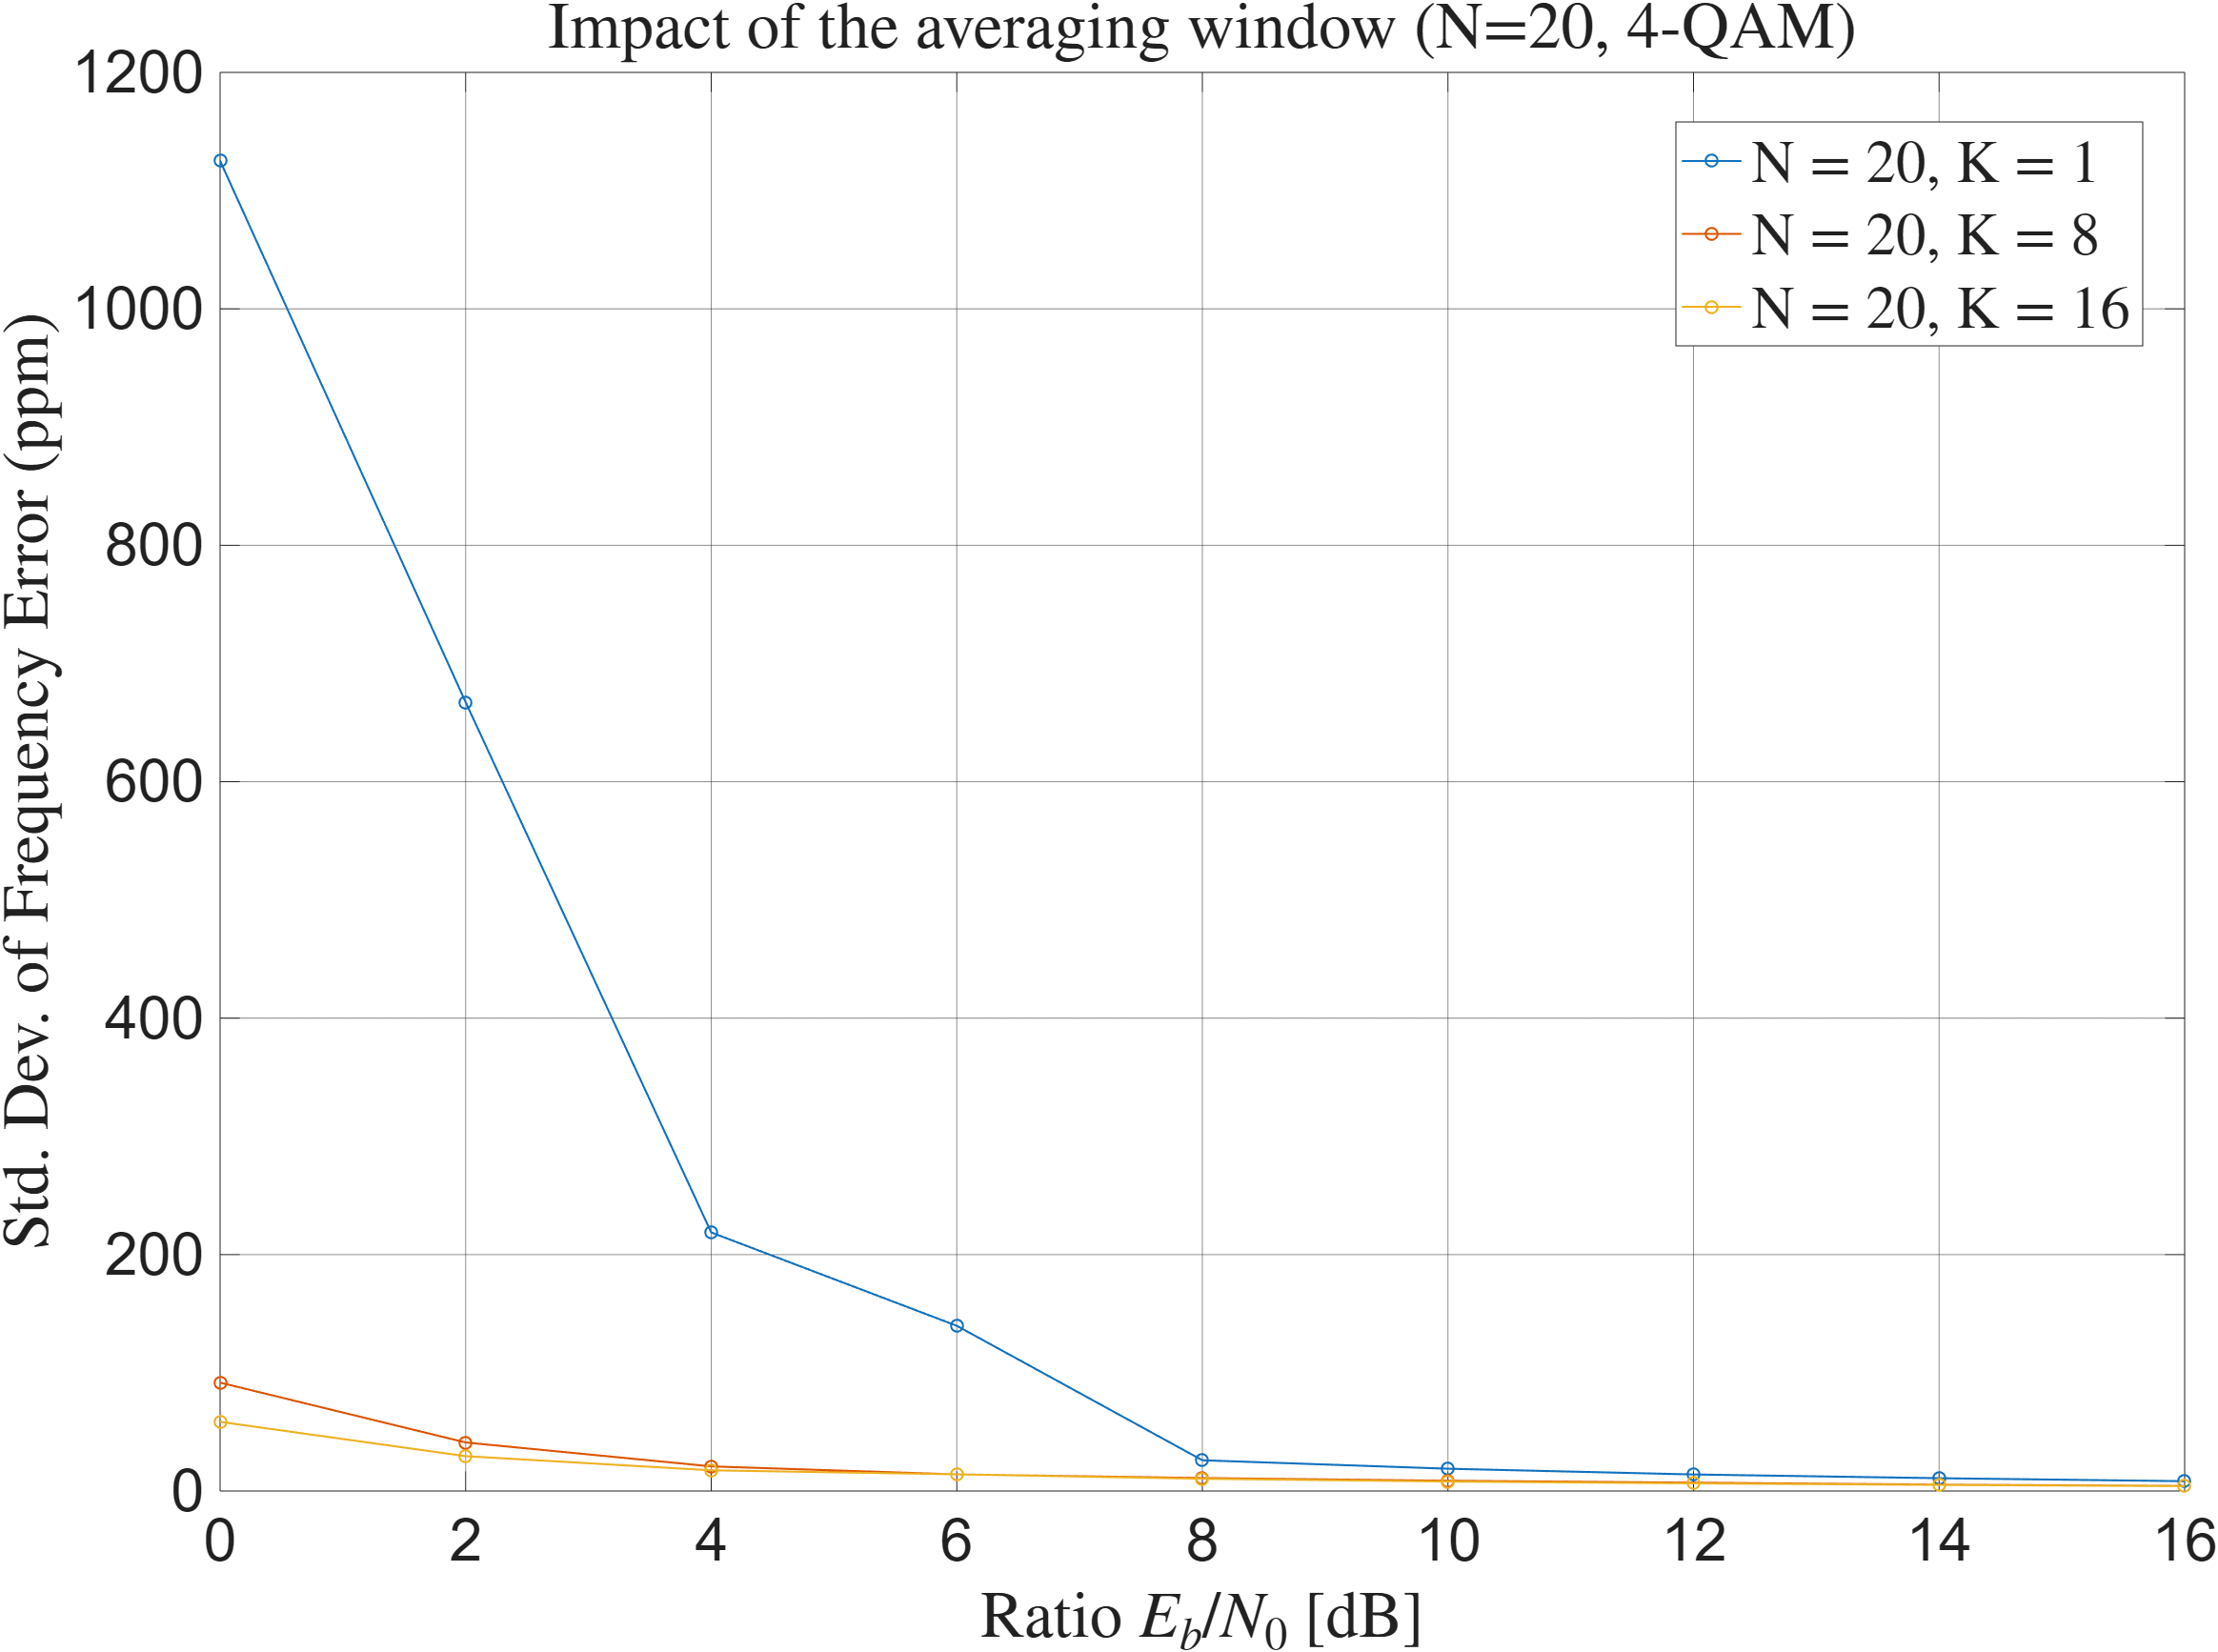
\includegraphics[width=\linewidth]{Images/cfo_est_K_avg.png} 
			\caption{CFO error std dev vs. $K$.}
		\end{subfigure}
		\caption{Acquisition error vs. $E_b/N_0$ for different averaging windows ($K$).}
		\label{fig:acquisition_vs_K_avg_compact}
	\end{figure}

	Further investigation into the robustness of the differential cross-correlator focuses on its performance in the presence of an existing CFO. Figure~\ref{fig:robustness-combined}(a) illustrates the standard deviation of the CFO estimation error against the $E_b/N_0$ ratio for various initial CFO values (0 ppm, 2 ppm, and 20 ppm) with a fixed timing offset $t_0 = 0.03T_{\text{symb}}$. The plot demonstrates that the CFO estimation accuracy improves with increasing $E_b/N_0$. Importantly, the performance is largely resilient to the initial CFO levels tested, with all three curves closely overlapping, indicating the estimator's robustness in accurately determining the CFO even when significant frequency offsets are already present.
	Similarly, the robustness of the Time of Arrival estimation to an existing CFO is presented in Figure~\ref{fig:robustness-combined}(b). This subfigure shows the standard deviation of the ToA error (in samples) as a function of $E_b/N_0$ under the same set of initial CFOs and timing offset. The ToA estimation performance significantly improves as $E_b/N_0$ increases, with the error dropping and then plateauing at very low levels for $E_b/N_0 > 2 \text{ dB}$. While the presence of a small initial CFO like 2 ppm has a negligible impact compared to the no-CFO case, a larger CFO (20 ppm) introduces a noticeable degradation, particularly at very low $E_b/N_0$ (around 0 dB), where the ToA error is higher. However, for $E_b/N_0$ values above approximately 2 dB, the ToA estimation remains highly accurate and robust even in the presence of a 20 ppm CFO.

	\begin{figure}[H]
		\centering
		\begin{subfigure}[b]{0.4\textwidth} 
			\centering
			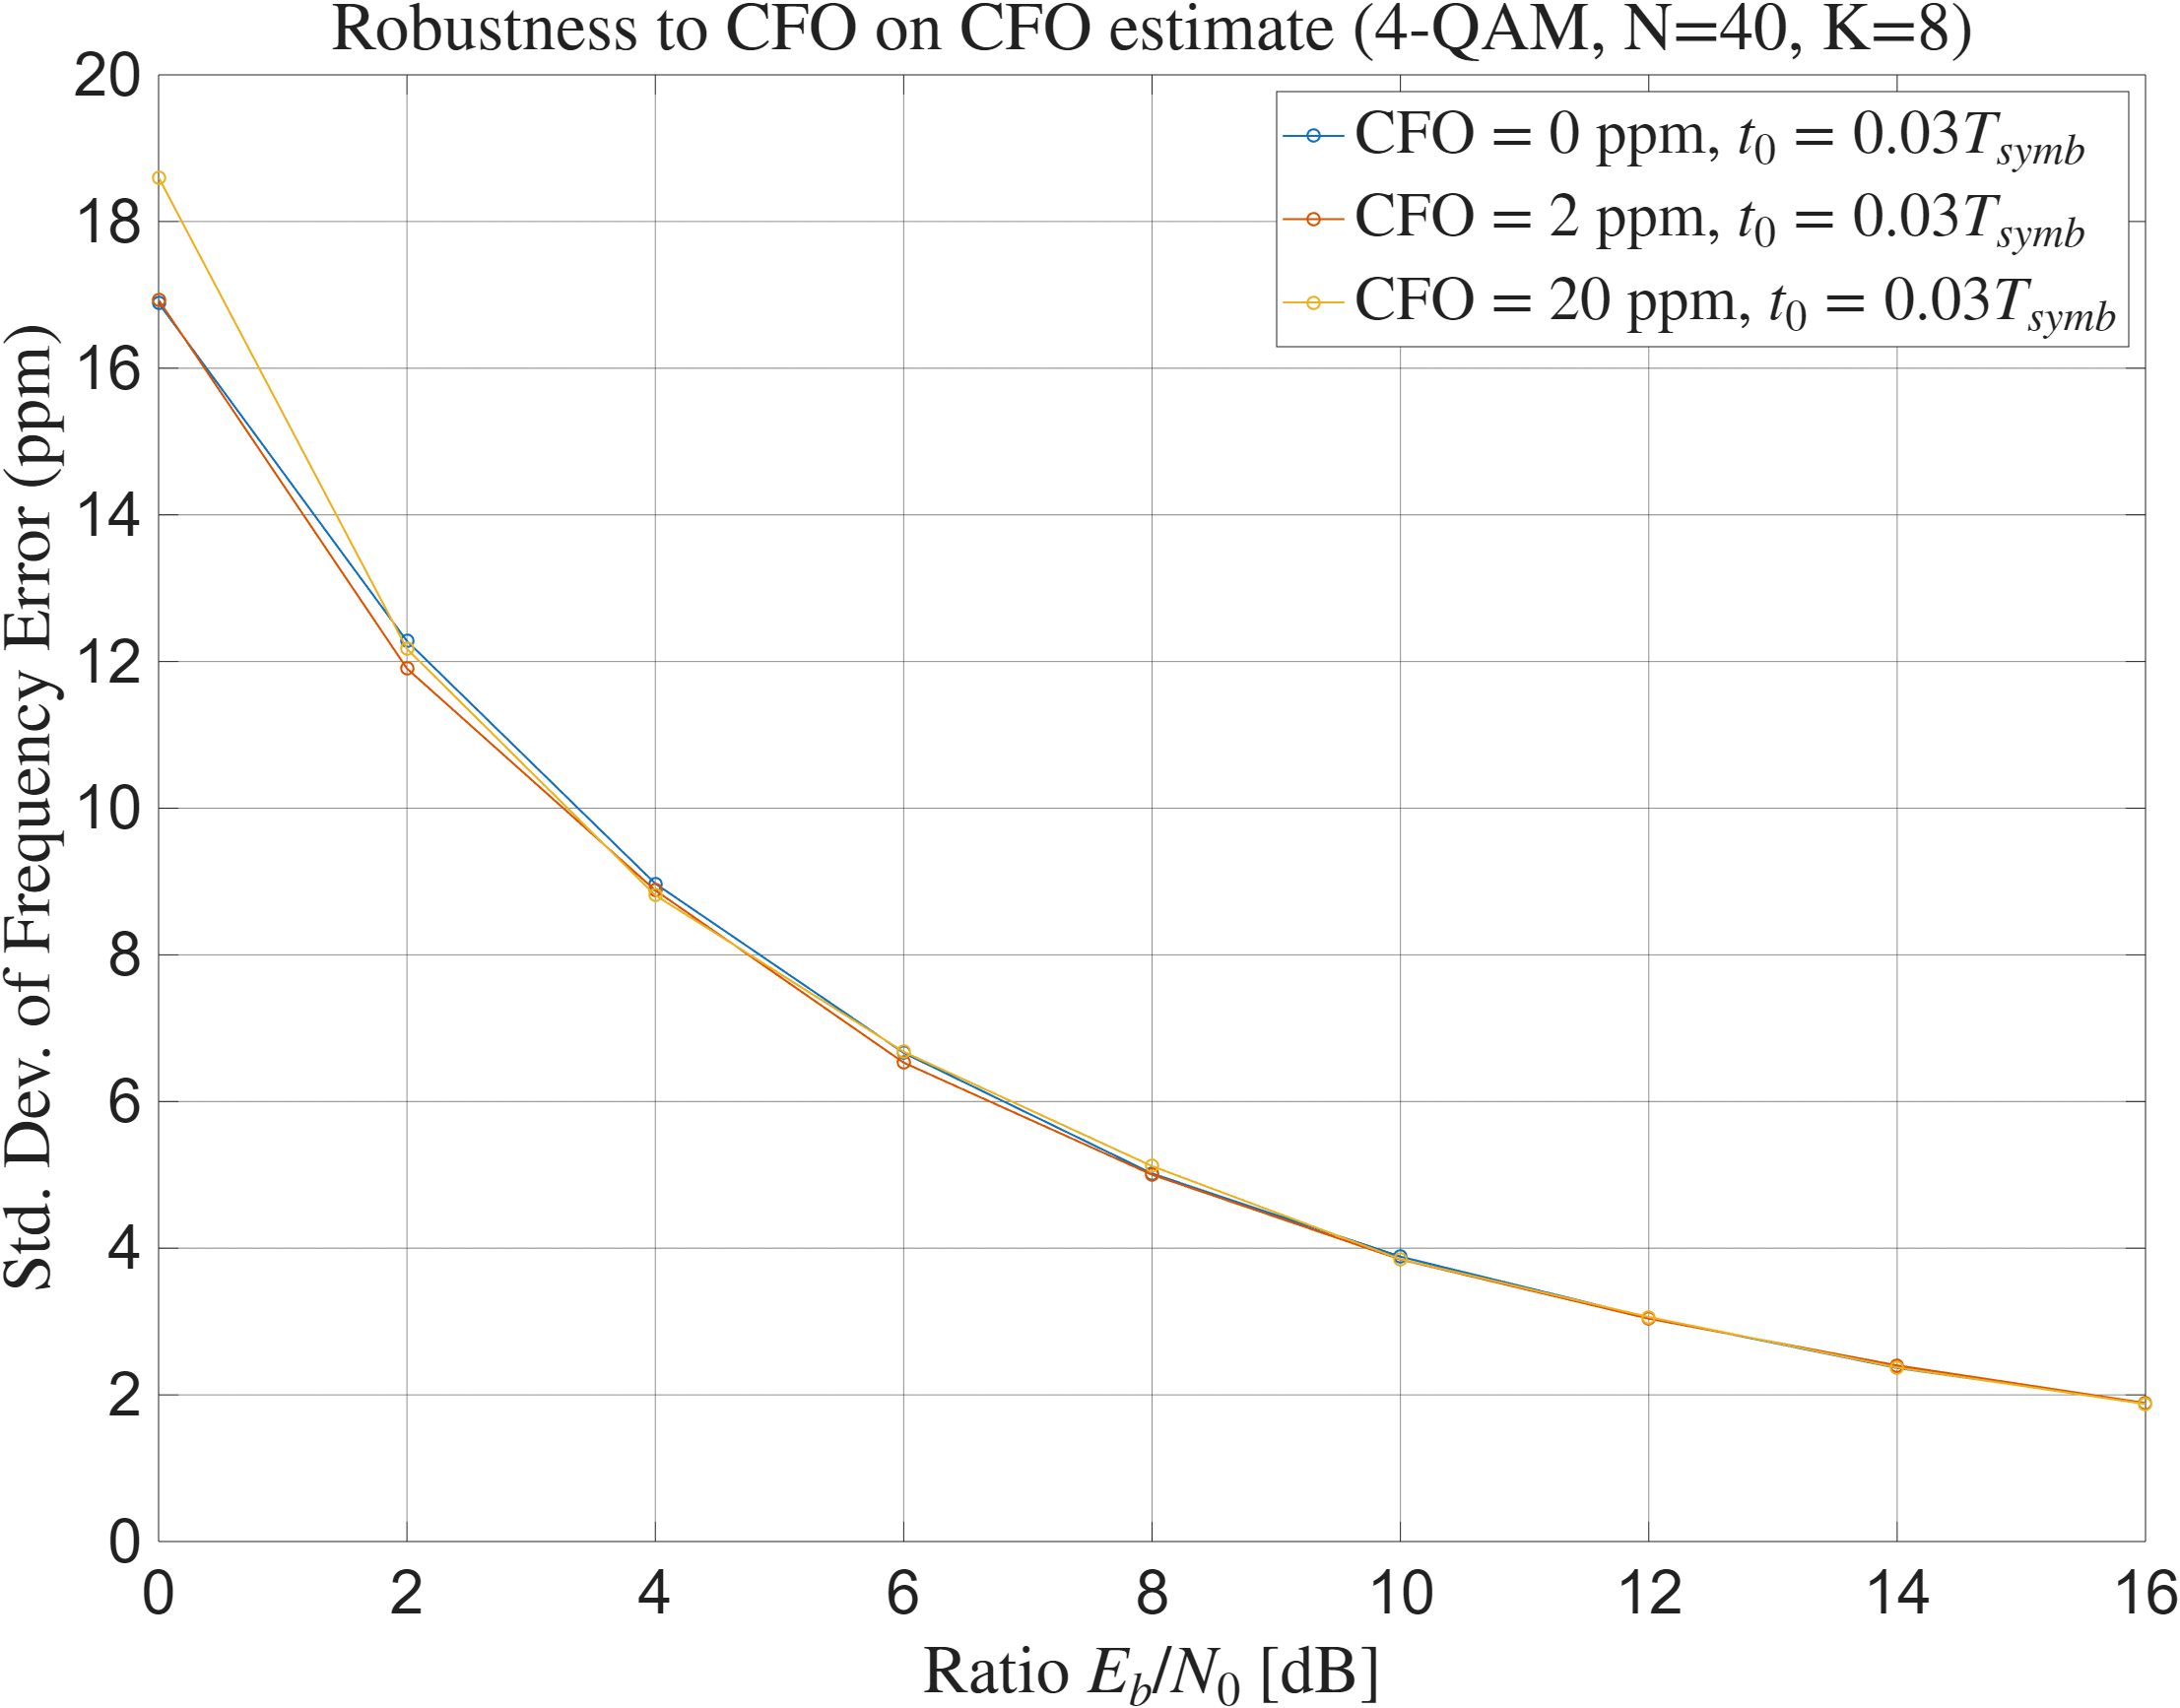
\includegraphics[width=\linewidth]{Images/robust-cfo.png}
			\caption{CFO estimation error vs. $E_b/N_0$.} 
			\label{fig:robust-cfo-sub}
		\end{subfigure}
		\hfill
		\begin{subfigure}[b]{0.4\textwidth} 
			\centering
			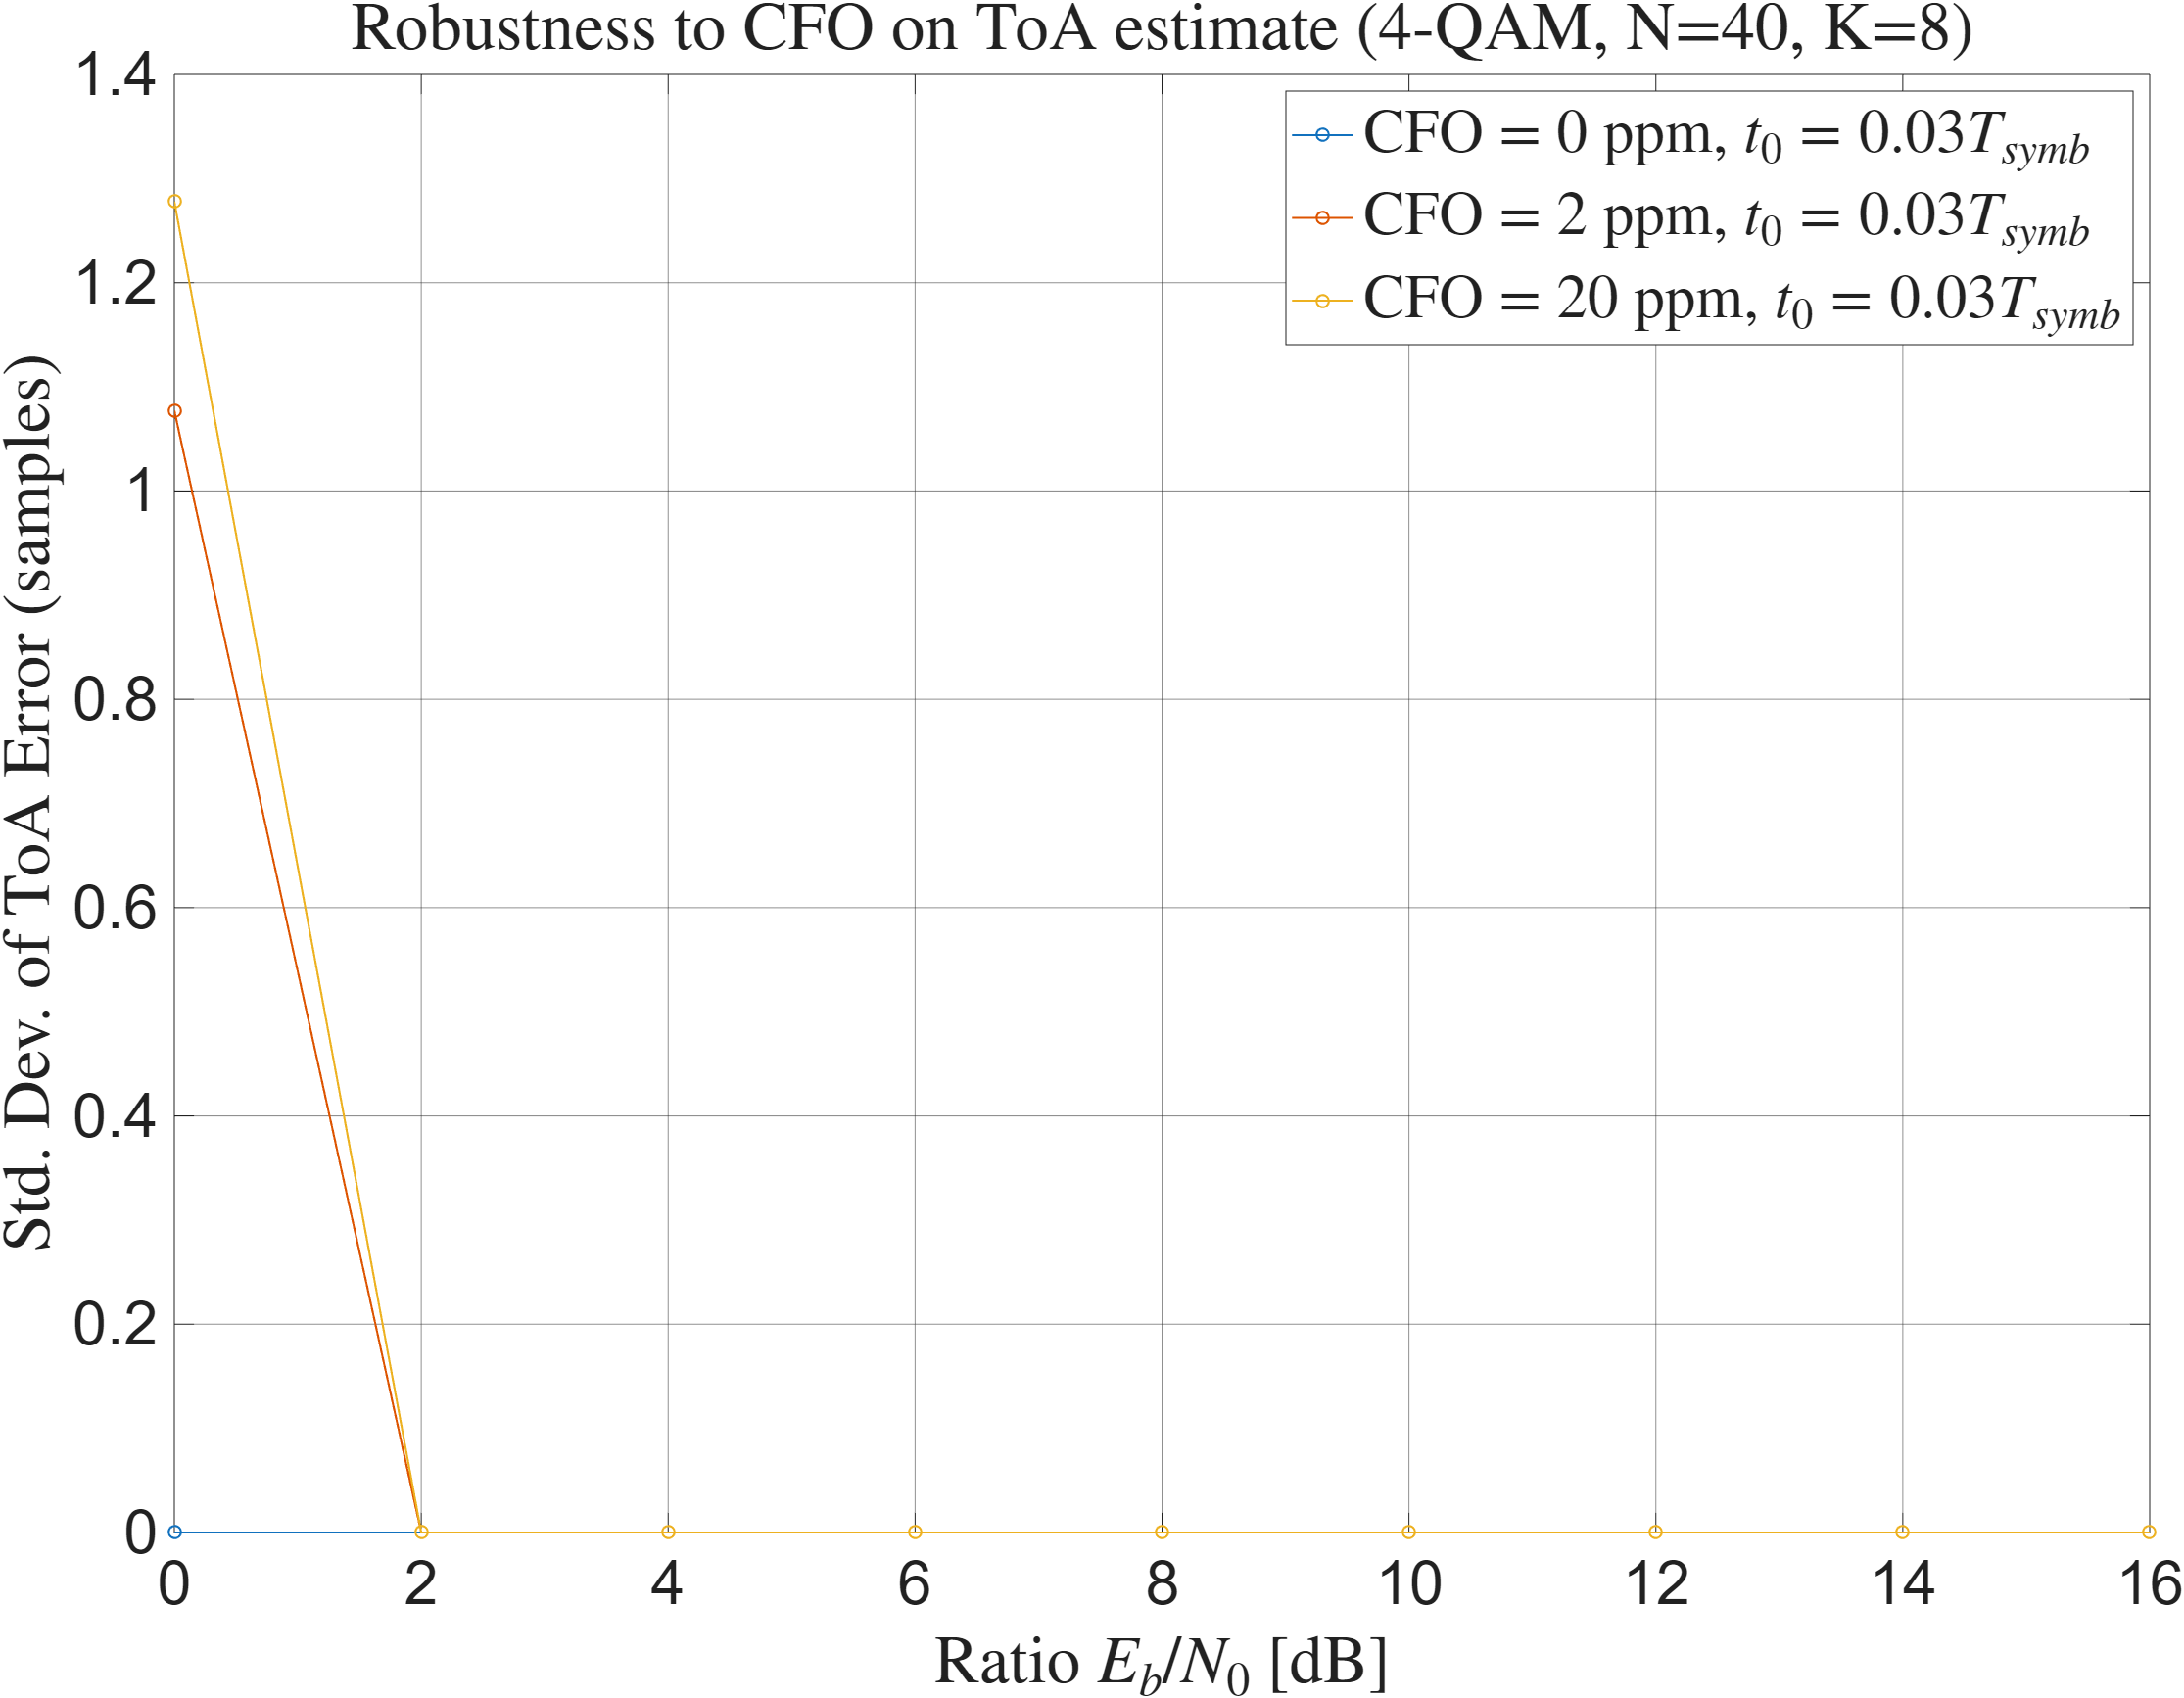
\includegraphics[width=\linewidth]{Images/robust-toa.png}
			\caption{ToA estimation error vs. $E_b/N_0$.} 
			\label{fig:robust-toa-sub}
		\end{subfigure}
		\caption{Robustness of CFO and ToA estimation to pre-existing CFO values (4-QAM, $N=40$, $K=8$, $t_0 = 0.03T_{\text{symb}}$).}
		\label{fig:robustness-combined}
	\end{figure}
	
        \subsection{Validation of the Communication chain}
        \begin{figure}[H]
		\centering
		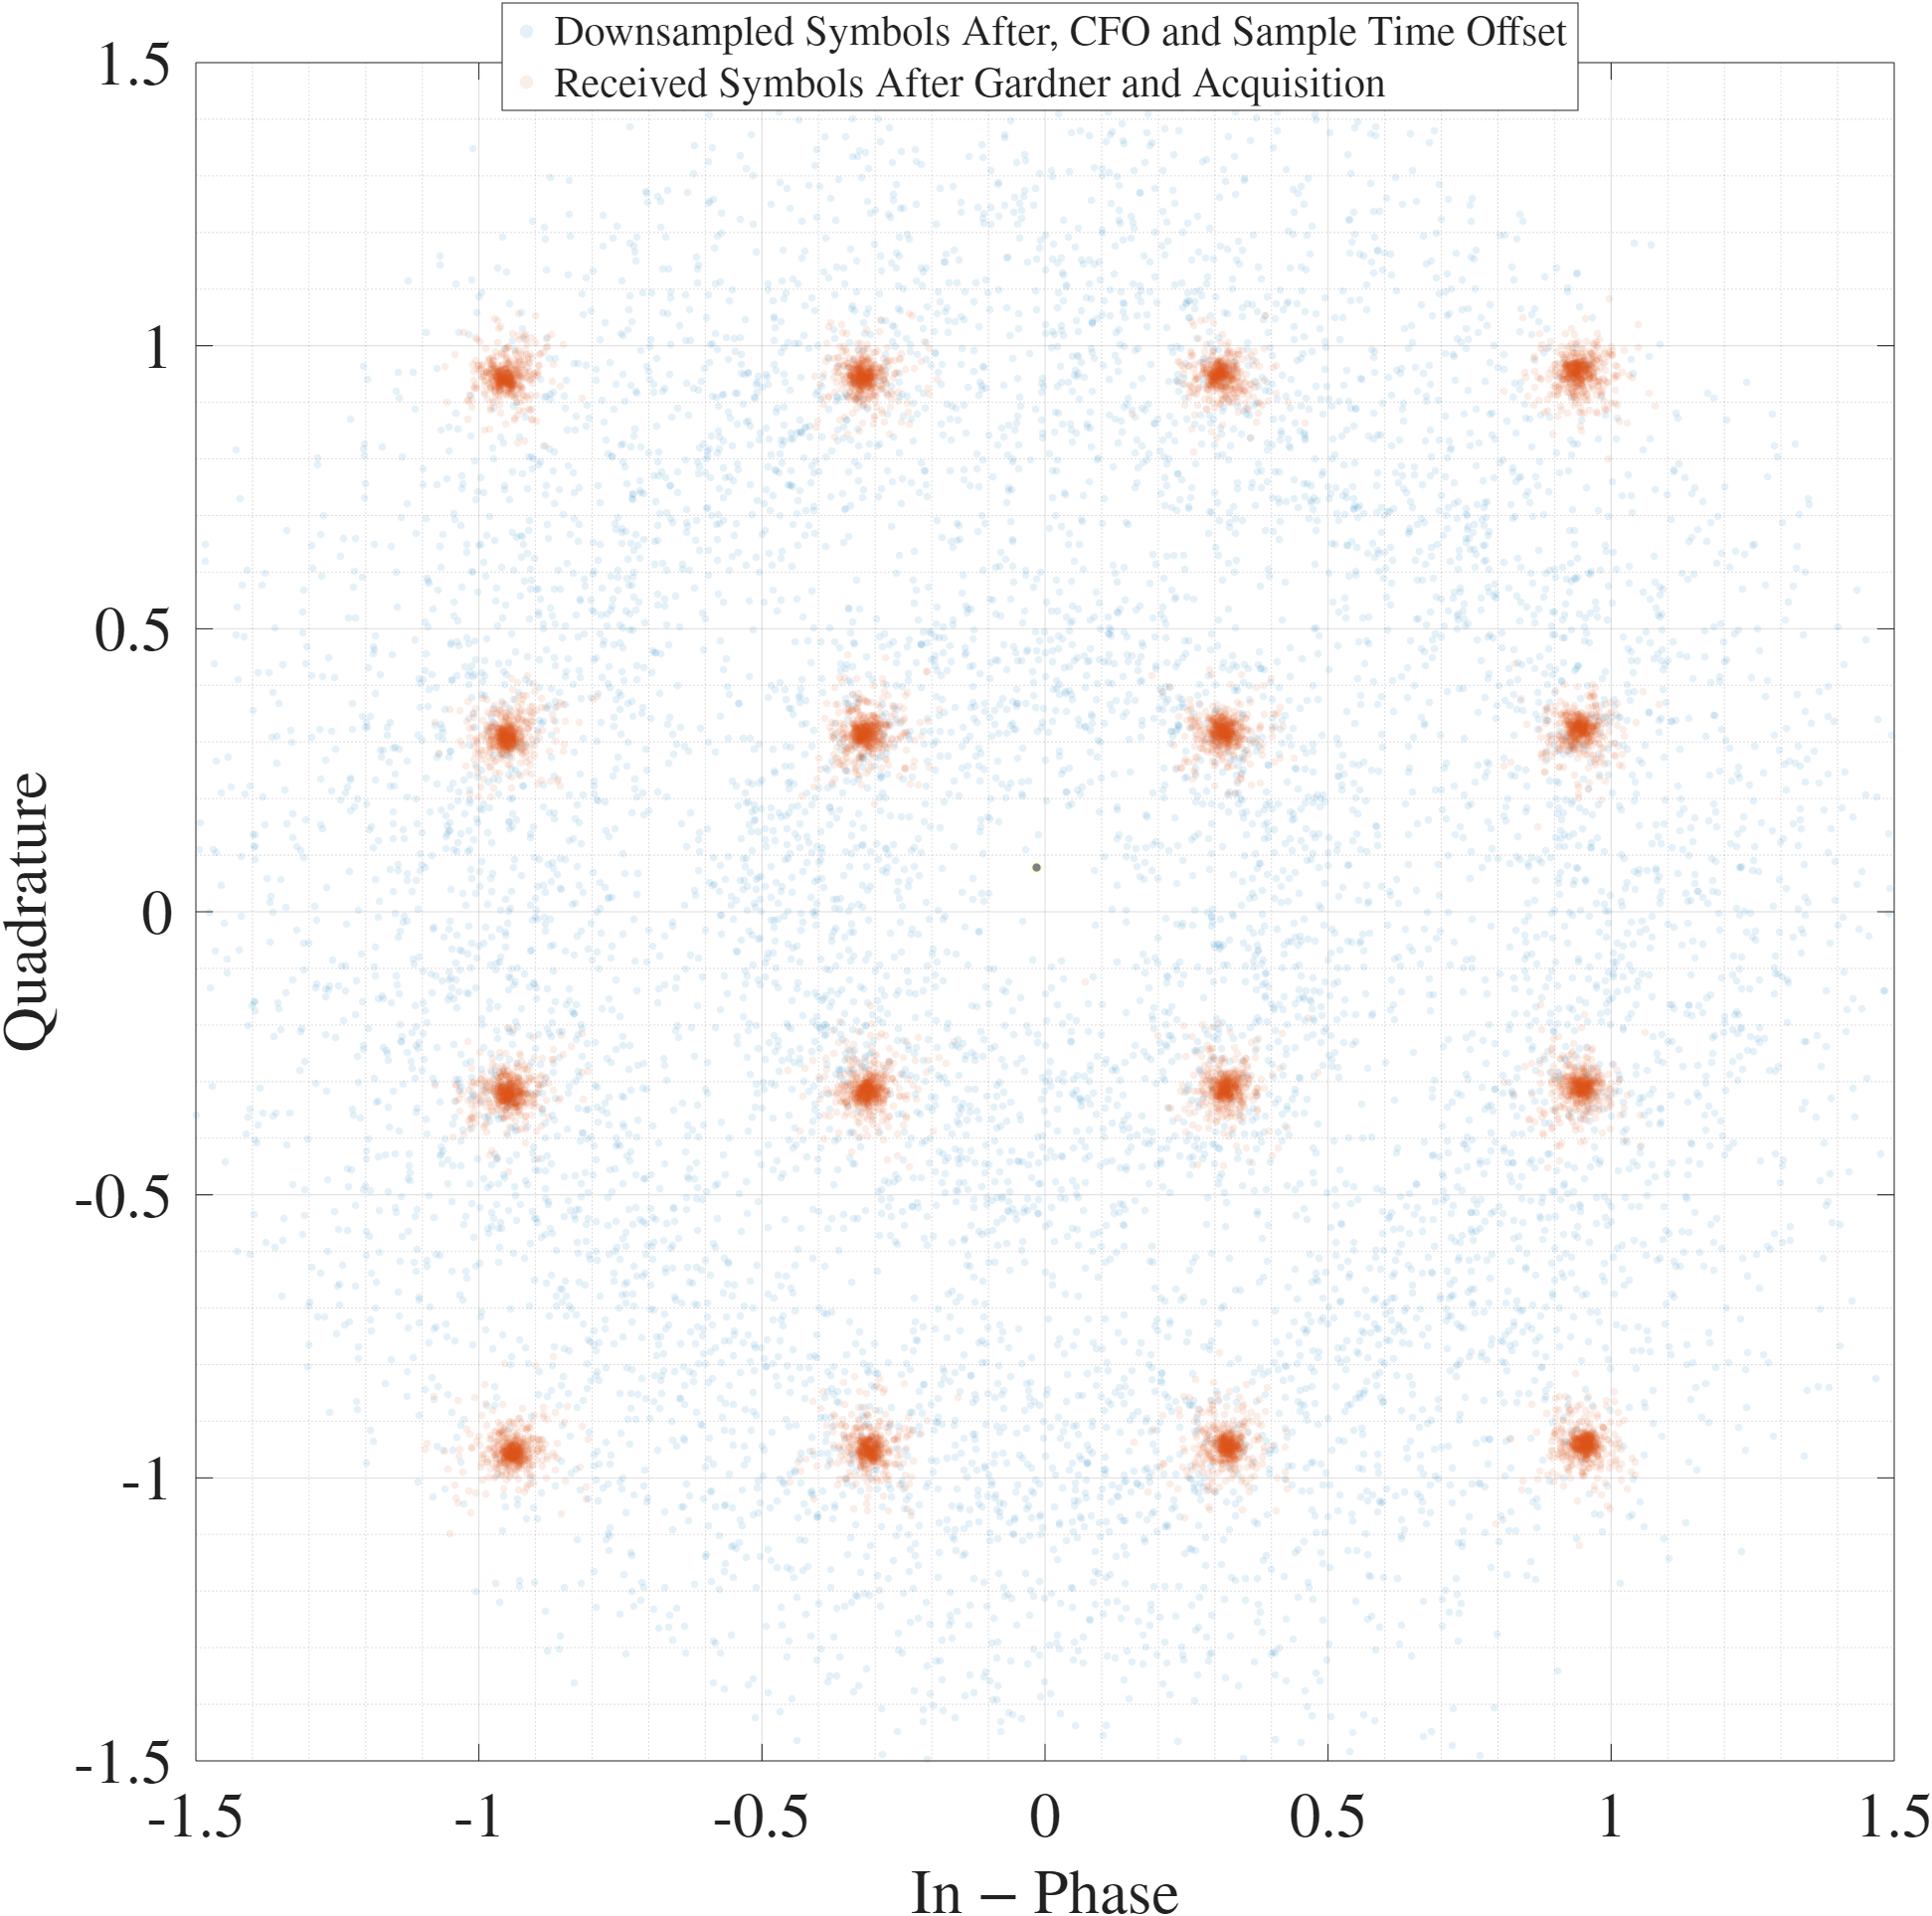
\includegraphics[width=0.55\linewidth]{Images/const-corrected.png} 
		\caption{16-QAM; No Noise; $\mathrm{CFO = 2 ppm}$; $\mathrm{t_0 = 0.1 T_{symb}}$; $\text{Numbits} = \text{Nbps} \times 2^{12}$; $\kappa = 0.1$; $\text{K} = 16$; $\mathrm{N = floor(length(symb_{tx}) \times 0.4)}$}
		\label{fig:const-corrected-after-sync}
	\end{figure}
        From the transmitter, to the receiver, the signal goes through each element of the communication chain. At the receiver, the synchronization pipeline is mainly: 1) Timing Recovery (Gardner), 2) Frame Acquisition, 3) Coarse CFO Acquisition 4) Compensation. This order ensures robustness. Figure \ref{fig:const-corrected-after-sync} visually confirms the significant improvement in constellation clarity after Gardner and Frame/CFO acquisition, thus validating the communication chain.
	
	
			
	\subsection{Questions: Time and Frequency Synchronization}
	\par\noindent\textbf{Derive analytically the baseband model of the channel including the synchronisation errors? :}\quad\ignorespaces 
		Received baseband signal is
		\begin{equation} \tilde{r}_e(t) = \tilde{s}(t-\epsilon T_{\text{symb}} - t_0) e^{j(2\pi\Delta f t + \phi_0)} \end{equation}
		where $\tilde{s}(t)$ is ideal transmitted baseband signal, $\epsilon$ is normalized clock offset, $t_0$ time shift, $\Delta f$ CFO, $\phi_0$ phase offset. For sampling at $nT_{\text{symb}}(1+\delta)+t_0'$, considering $y[n]$ as output of matched filter and ADC.
	\par
			
	\par\noindent\textbf{How do you separate the impact of the carrier phase drift and ISI due to the CFO in your simulation? :}\quad\ignorespaces 
		Phase drift from CFO is 
		\begin{equation} e^{j2\pi \Delta f nT_{\text{symb}}} \end{equation}
		on symbols $I[n]$. ISI results from $g(t)e^{j2\pi\Delta ft}$ convolved with $g^*(-t)$ not being a perfect Nyquist pulse. To see ISI alone, multiply received symbols by 
		\begin{equation} e^{-j2\pi \Delta f nT_{\text{symb}}} \end{equation}
		after matched filtering to remove coherent phase rotation, then observe BER degradation.
	\par
			
	\par\noindent\textbf{How do you simulate the sampling time shift in practice? :}\quad\ignorespaces 
		Increase sampling rate by large factor $M_{\text{os}}$ pre-filter. A shift of $k$ samples at this high rate corresponds to
		\begin{equation} t_0 = k \cdot \frac{T_{\text{symb}}}{M_{\text{os}}} \end{equation}
		Alternatively, use interpolation on the oversampled signal at the receiver output to estimate values at $nT_{\text{symb}} + t_0$.
	\par
			
	\par\noindent\textbf{How do you select the simulated $E_b/N_0$ ratio? :}\quad\ignorespaces 
		$E_b/N_0$ must be high enough for synchronization algorithms to lock and provide meaningful performance metrics without being dominated by noise failures. Typically, choose values where uncoded BER is reasonably low (e.g., $10^{-2}$ to $10^{-4}$), or a typical operating point. For some algorithms, a minimum $E_b/N_0$ (e.g., > 4-6 dB) is needed for reliable acquisition, as seen in frame/frequency acquisition plots.
	\par
			
	\par\noindent\textbf{How do you select the lengths of the pilot and data sequences? :}\quad\ignorespaces 
		Pilots ($N$): Long enough for accurate ToA/CFO/Phase estimation against noise (e.g., $N \ge 20-40$). Too short leads to high estimation variance.
		Data: Short enough between pilots to ensure phase drift from residual CFO is < $\pi$ and linear phase change assumption holds.
		Trade-off: Longer/more frequent pilots improve sync but reduce data throughput (overhead).
	\par
			
	\par\noindent\textbf{In which order are the synchronisation effects estimated and compensated? Why? :}\quad\ignorespaces 
		1. Timing Recovery (Gardner): Robust to CFO.
		2. Frame/Frequency Acquisition (Differential Cross-correlator): Uses timed samples to find frame start and correct large CFO.
		This order allows each stage to operate on a signal pre-processed to mitigate errors that would impair its own performance.
	\par
			
	\par\noindent\textbf{Explain intuitively how the error is computed in the Gardner algorithm. Why is the Gardner algorithm robust to CFO? :}\quad\ignorespaces 
		The error is:
		\begin{equation} e[n] = \operatorname{Re} \{ y[n-1/2] ( y^{*}[n] - y^{*}[n-1] ) \} \end{equation}
		$y[n-1/2]$ is the mid-point sample. $(y^{*}[n] - y^{*}[n-1])$ estimates signal slope. If $y[n-1/2]$ and slope have same sign, timing is late; opposite sign, early. No transition means small slope, small update.
		Robustness to CFO: CFO causes phase rotation
		\begin{equation} \Delta\phi = 2\pi \Delta f T_{\text{symb}} \end{equation}
		between $y[n-1]$ and $y[n]$, and $\Delta\phi/2$ on $y[n-1/2]$. The error term uses $\operatorname{Re}\{\cdot\}$. For small $\Delta\phi$ per symbol (typical CFOs),
		\begin{equation} e^{j\Delta\phi} \approx 1+j\Delta\phi \end{equation}
		The dominant terms in the error calculation are less affected by these small phase rotations.
	\par
			
	\par\noindent\textbf{Explain intuitively why the differential cross-correlator is better suited than the usual cross-correlator? Isn't interesting to start the summation at $k=0$ (no time shift)? :}\quad\ignorespaces 
		Usual cross-correlator 
		\begin{equation} C[n] = \sum y^*[n+l]a[l] \end{equation}
		is sensitive to CFO, as CFO rotates $y[n+l]$ causing phase terms 
		\begin{equation} e^{j2\pi\Delta f (n+l)T_{\text{symb}}} \end{equation}
		that don't cancel in $|C[n]|$, degrading the peak.
		Differential cross-correlator (Eq. \ref{eq:diff_corr_metric_style_change}) multiplies two correlation terms with a time lag $k$. The product 
		\begin{equation} (y^*[n+l]a[l])(y[n+l-k]a^*[l-k]) \end{equation}
		has phase
		\begin{equation} e^{-j2\pi\Delta f(n+l)T_{\text{symb}}} \cdot e^{j2\pi\Delta f(n+l-k)T_{\text{symb}}} = e^{-j2\pi\Delta f k T_{\text{symb}}} \end{equation}
		The phase is proportional to $k\Delta f$, allowing $\Delta f$ estimation. The magnitude is less affected by the absolute phase.
		Summation for $k=0$:
		\begin{equation} D_0[n] = \frac{1}{N}\sum |y[n+l]a[l]|^2 \end{equation}
		which relates to energy detection but doesn't directly use the differential property for CFO estimation. The CFO estimation relies on $k \ge 1$.
	\par
			
	\par\noindent\textbf{Are the frame and frequency acquisition algorithms optimal? If yes, give the optimisation criterion? :}\quad\ignorespaces 
		The ML criterion for joint ToA ($\hat{n}$) and CFO ($\Delta\omega$) estimation is
		\begin{equation} (\hat{n},\Delta\omega)= \operatorname*{arg\,max}_{n,\omega} p(y[n]|a,\Delta\omega) \end{equation}
		Direct implementation is complex (2D search over $n$ and $\omega$). The differential cross-correlator is a near-optimal, lower-complexity approximation. It's not strictly ML optimal because it simplifies the likelihood function or uses derived metrics, often omitting terms like received signal power that an exact ML estimator might include.
	\par

        \section{Orange Seminar Questions}
        \subsection{HFC Architecture, Main Components, and Capacity Bottleneck}
        \noindent\textbf{Question: Describe the architecture of the HFC network and its main components. Where is the capacity bottleneck today?}
        
        The Hybrid Fiber-Coax network combines fiber optic and coaxial cables. The headend aggregates signals for transmission. In HFC, the headend includes an optical node converting optical to electrical signals for coax transmission and vice versa. Fiber cables are used for long-distance, large-capacity transmission from servers and data sources. Coaxial cables connect to households, with passive taps splitting the signal. RF amplifiers are placed to boost signals attenuated by losses.
        
        The primary capacity bottleneck in current HFC networks is in the upstream direction. Upstream bandwidth is often limited to around 150 MHz supporting 1 to 2 Gbps, while downstream may have 1000 MHz allowing up to 10 Gbps. This asymmetry constrains upstream capacity. Shared bandwidth in the coaxial part and the need for equipment upgrades also contribute to bottlenecks.
        
        \subsection{Future Evolution of HFC Networks and Key Technologies}
        \noindent\textbf{Question: What will be the evolution of the HFC network in the coming years? What are the key technologies to make this happen?}
        
        HFC networks will evolve to support higher bandwidths, lower latency, and improve energy efficiency. This evolution will occur in parallel with Fibre To The Premises deployments. The HFC network will use more fiber to extend bandwidth, speed, and reliability.
        
        Key technologies driving this evolution include DOCSIS 4.0, which encompasses Extended Spectrum DOCSIS and Full Duplex DOCSIS. Distributed Access Architecture, using Remote PHY or Remote MAC-PHY, moves digital processing closer to users, replacing RF over fiber with Ethernet/IP. Node splitting and fibre deepening will reduce homes per optical node, increasing bandwidth per user. Integration with FTTP solutions like XGS-PON and 50G-PON is also a key aspect. Advanced modems and Wi-Fi 6/7 will support multi-gigabit speeds.
        
        \subsection{Typical Incidents on Orange's Network and Mitigation Procedures}
        \noindent\textbf{Question: Which are the typical incidents happening on Orange's network? Explain the procedure foreseen to cope with them.}
        
        Typical incidents on Orange's network are often due to construction works, where digging can accidentally damage underground cables and infrastructure. Damaged wires underground are another common issue.
        
        To cope with these, fault locations are estimated, for instance, by timing fiber signals. Repairs for physical disruptions can take at least a few hours. For critical locations such as hospitals and emergency services, redundant lines or backup connections are installed to ensure continuous connectivity. Reconstruction works for high-priority objects are done faster. Active traffic monitoring and capacity management using past data and machine learning are also employed to ensure service continuity.
        
        \subsection{Orange Data Center Characteristics}
        \noindent\textbf{Question: Describe the main Orange's data center in numbers (storage, in/out capacity, consumed power, area, maintenance...).}
        
        The Orange data center has a maximum power capacity of 3 MW and currently operates at approximately 1.5 MW. It uses 400 V AC and 48 V DC power distribution systems. The facility employs passive cooling techniques with six cooling blocks and has additional space reserved for future cooling expansion.
        
        For backup power, there are two generators, each rated at 750 kW. A fuel tanker can supply energy for up to 72 hours in emergencies. The average transmission rate is in the order of terabytes per second. The center also has redundant area for scaling and reliability.
    			
\end{document}